\chapter{Diffusion Models Today: Score SDE Framework}\label{ch:score-sde}

\epigraph{
    \textit{There is only one precise way of presenting the laws, and that is by means of differential equations. They have the advantage of being fundamental and, so far as we know, precise.
}}{Richard P. Feynman}



So far, we have studied diffusion models from two perspectives: the variational view and the score-based view, the latter naturally emerging from the EBM formulation. We now take the next step and move to the \emph{continuous-time framework}. At its core lies the \emph{Score SDE}, the continuous limit that unifies DDPM and NCSN into a single formulation. This perspective is powerful because it extends discrete updates with a clean, principled description grounded in differential equations (DE).
In this view, generation reduces to solving a DE over time. This lets us directly apply tools from numerical analysis: for example, the basic Euler method can simulate the dynamics, while more advanced solvers improve stability and efficiency.
By working in continuous time, we also gain a richer mathematical structure and a unified foundation for understanding, analyzing, and improving diffusion models. This perspective will be developed further in this monograph.






\newpage

\section{Score SDE: Its Principles}\label{sec:dm-today}
% The use of multiple noise scales has been a crucial ingredient in the success of NCSN and DDPM frameworks. In this section, we introduce the foundation of the \emph{Score SDE}~\citep{song2020score}, which elevates this idea by considering a continuum of noise levels which this continuous-time limit of forward/reverse diffusion model perspective had been pointed out in \citep{sohl2015deep}. Instead of perturbing data using a fixed or finite set of noise magnitudes, \citet{song2020score} propose a formulation in which the data distribution evolves smoothly over time according to an SDE, as the noise level continuously increases. This continuous-time perspective not only unifies prior discrete models, but also enables a principled and flexible framework for generative modeling via continuous-time processes.
\begin{figure}
    \centering
    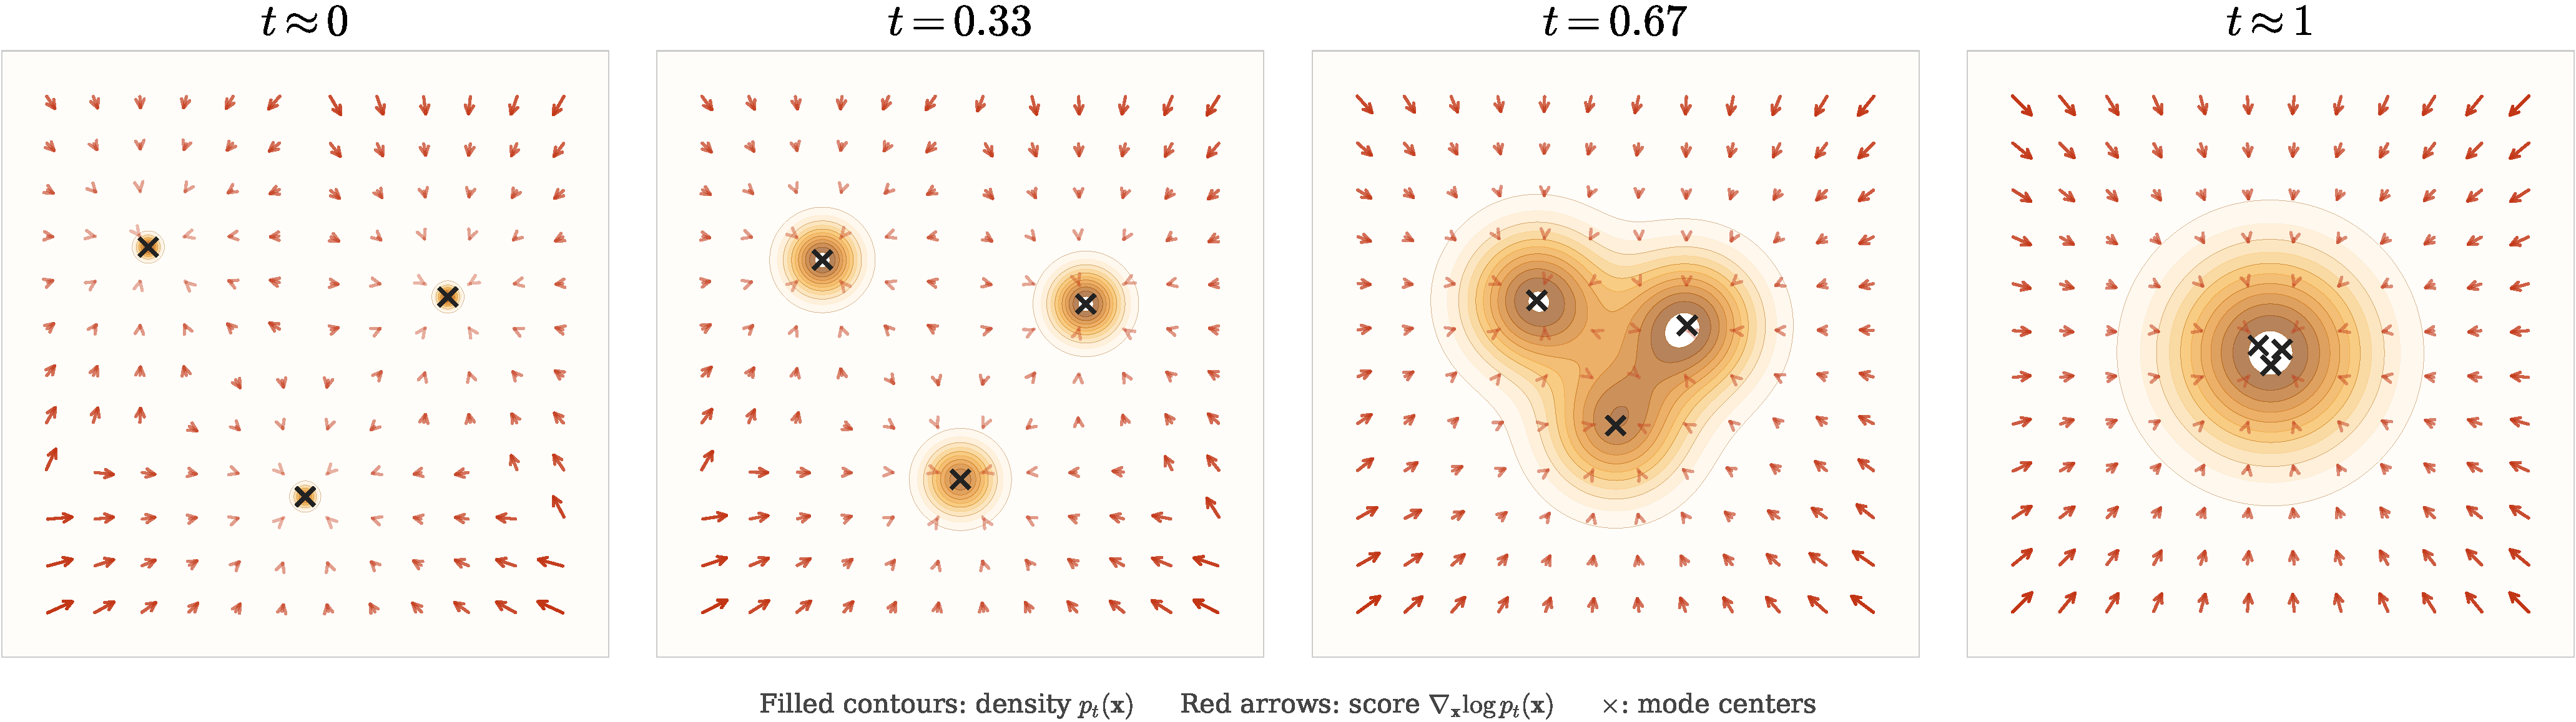
\includegraphics[width=\linewidth]{Images/PartB/score_landscape_2d.pdf}
    \caption{\textbfs{Illustration of the time-dependent score landscape.}
As the noise level increases, the perturbed density $p_t(\rvx)$ evolves from a multimodal distribution (data) concentrated near the data modes to a broad nearly unimodal distribution (prior).
Accordingly, the score field $\nabla_{\rvx}\log p_t(\rvx)$ changes from a sharply local vector field that pulls samples toward nearby modes to a smooth global field that points toward the overall center of mass.
This time-dependent score field is the key object learned in score-based diffusion models (i.e., Score SDE). \figcredit{Created by the authors with AI-assisted coding.}}
    \label{fig:time-dependent-score}
\end{figure}

% The use of multiple noise scales has been a crucial ingredient in the success of NCSN and DDPM frameworks. In this section, we introduce the foundation of the \emph{Score SDE}~\citep{song2020score}, which elevates this idea by considering a continuum of noise levels. A continuous-time limit of forward and reverse diffusion processes had already been noted by \citet{sohl2015deep}, but \citet{song2020score} make this perspective central by formulating the data evolution as a stochastic/ordinary differential equation, where the noise level increases smoothly over time. This continuous-time formulation not only unifies prior discrete-time models but also provides a principled and flexible foundation for generative modeling by casting it as the problem of solving differential equations.

The use of multiple noise scales has been a crucial ingredient in the success of NCSN and DDPM frameworks. In this section, we introduce the foundation of the \emph{Score SDE}~\citep{song2020score}, which elevates this idea by considering a continuum of noise levels. A continuous-time limit of forward and reverse diffusion processes had already been noted by \citet{sohl2015deep}, but \citet{song2020score} make this perspective central by formulating the data evolution as a stochastic/ordinary differential equation, where the noise level increases smoothly over time. Central to this formulation is the \emph{time-dependent score function} $\nabla_{\rvx}\log p_t(\rvx)$: at each noise level~$t$, it points toward regions of higher density under the current noisy distribution~$p_t$, and it is precisely this quantity that determines how to reverse the diffusion. As \Cref{fig:time-dependent-score} illustrates, the score field evolves from sharply converging toward individual data modes at small~$t$ to pointing gently toward the global center at large~$t$. This continuous-time formulation not only unifies prior discrete-time models but also provides a principled and flexible foundation for generative modeling: learning this family of score functions across all noise levels reduces generation to the problem of solving differential equations.




% \se{might need to properly attribute the 2015 paper, they had a continuous time version there}

% \jcr{The use of multiple noise scales has been central to NCSN and DDPM. In this section we adopt the continuous-time view popularized by the \emph{Score SDE}~\citep{song2020score}, which models a continuum of noise levels via an SDE. A continuous-time perspective predates this:  provided  continuous-time limit and time-reversal perspective of variational-based diffusion model. Building on that foundation, \citet{song2020score} make the reverse-time dynamics explicit in terms of the score $\nabla_{\rvx}\log p_t(\rvx)$, thereby unifying DDPM and SMLD and enabling principled sampling with SDE/ODE solvers. We focus on this score-driven formulation below.
% }

\subsection{Motivation: From Discrete to Continuous-Time Processes}\label{subsec:scoresde-motivation}

% \se{either reintroduce the symbols, or refer to previous equations. i would probably reintroduce if you expect people to skip chapters}
We revisit the forward noise injection schemes of NCSN and DDPM. NCSN uses a sequence of increasing noise levels $\{\sigma_i\}_{i=1}^L$. 
Each clean sample $\rvx_0 \sim p_{\mathrm{data}}$ is perturbed as
\[
\rvx_{\sigma_i} = \rvx_0 + \sigma_i \bm{\epsilon}_i, 
\qquad \bm{\epsilon}_i \sim \mathcal{N}(\bm{0}, \rmI).
\]
DDPM instead injects noise incrementally with a variance schedule $\{\beta_i\}_{i=1}^L$\footnote{In \Cref{sec:ddpm}, the DDPM forward step is written as $\rvx_i = \sqrt{1-\beta_i^2}\,\rvx_{i-1} + \beta_i\,\bm{\epsilon}_i$, where $\beta_i$ denotes the standard deviation of the injected noise and $\alpha_i := \sqrt{1-\beta_i^2}$. Here and throughout this chapter, we follow the convention of \citet{song2020score}, where $\beta_i$ instead denotes the variance of the injected noise, so that $\rvx_i = \sqrt{1-\beta_i}\,\rvx_{i-1} + \sqrt{\beta_i}\,\bm{\epsilon}_i$. The two conventions are related by $\beta_i^{\textup{(here)}} = \bigl(\beta_i^{\textup{(Ch.\ \ref{ch:variational})}}\bigr)^2$ and yield identical dynamics.}:
\[
\rvx_i = \sqrt{1 - \beta_i}\, \rvx_{i-1} + \sqrt{\beta_i}\, \bm{\epsilon}_i, 
\qquad \bm{\epsilon}_i \sim \mathcal{N}(\bm{0}, \rmI).
\]

We view them together on a discrete time grid, where the sequential update from $\rvx_t$ to $\rvx_{t+\Delta t}$ takes the form\footnote{For convenience, we use $\rvx(t)$ and $\rvx_t$ interchangeably (and similarly for other time-dependent variables) to denote samples at time $t$.}:
\begin{align*}
    \text{\textbfs{NCSN:}} \,\,
    & \rvx_{t+\Delta t} = \rvx_t + \sqrt{\sigma_{t+\Delta t}^2 - \sigma_t^2} \bm{\epsilon}_t 
    &&\approx \rvx_t + \sqrt{\frac{\diff \sigma_t^2}{\diff t} \Delta t}  \bm{\epsilon}_t \\[0.5em]
    \text{\textbfs{DDPM:}} \,\,
    & \rvx_{t+\Delta t} = \sqrt{1 - \beta(t)\Delta t} \rvx_t + \sqrt{\beta(t)\Delta t} \bm{\epsilon}_t 
    &&\approx \rvx_t - \frac{1}{2} \beta(t) \rvx_t  \Delta t + \sqrt{\beta(t)\Delta t}  \bm{\epsilon}_t,
\end{align*}
where $\bm{\epsilon}_t \sim \mathcal{N}(\bm{0}, \rmI)$. Interestingly, both noise injection processes follow a common structural pattern:
\begin{align}\label{eq:euler-discrete-sde}
    \rvx_{t+\Delta t} \approx \rvx_t + \rvf(\rvx_t, t) \Delta t + g(t) \sqrt{\Delta t}\, \bm{\epsilon}_t,
\end{align}
with $\rvf: \mathbb{R}^D \times \mathbb{R} \to \mathbb{R}^D$ and $g: \mathbb{R} \to \mathbb{R}$ given by:
\begin{align*}
    \text{\textbfs{NCSN:}} \quad 
    & \rvf(\rvx, t) = 0, \qquad g(t) = \sqrt{\frac{\diff \sigma^2(t)}{\diff t}} \\[0.5em]
    \text{\textbfs{DDPM:}} \quad 
    & \rvf(\rvx, t) = -\frac{1}{2} \beta(t)\, \rvx, \qquad g(t) = \sqrt{\beta(t)}.
\end{align*}


\begin{figure}
    \centering
    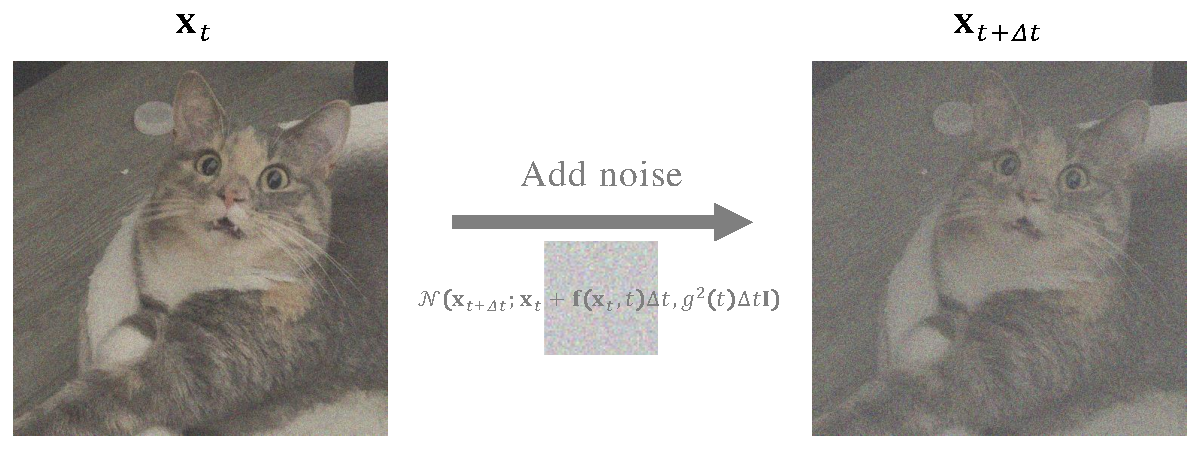
\includegraphics[width=0.9\linewidth]{Images/PartB/sde-forward-noise.pdf}
    \caption{\textbfs{Illustration of the discrete-time noise-adding step.} It adds noise from $t$ to $t + \Delta t$ with mean drift $\rvf(\rvx_t, t)$ and diffusion coefficient $g(t)$. \figcredit{Created by the authors.}}
    \label{fig:sde-forward-noise}
\end{figure}

This formulation corresponds to the following Gaussian transition:
\begin{align}\label{eq:transition-forward-f-g}
    p(\rvx_{t+\Delta t} |\rvx_t) := \mathcal{N}\!\left(\rvx_{t+\Delta t}; \rvx_t + \rvf(\rvx_t, t)\Delta t,\, g^2(t)\Delta t\, \rmI\right),
\end{align}
where, by a slight abuse of notation, we treat $\rvx_t$ as a fixed sample and $\rvx_{t+\Delta t}$ as a random variable.

As $\Delta t \to 0$ (which can be conceptually understood as preparing \emph{infinitely many} layers of noises), the discrete-time process converges to a continuous time SDE evolving forward in time\footnote{The forward kernel in \Cref{eq:transition-forward-f-g} converges, as $\Delta t\to0$, to the solution of the corresponding Itô SDE. A fully rigorous proof relies on advanced results which we defer to the literature.}:
\begin{align*}
    \diff \rvx(t) = \rvf(\rvx(t), t) \diff t + g(t) \diff \rvw(t),
\end{align*}
where $\rvw(t)$ is a standard Wiener process (or Brownian motion).
\rmkb{While a full formal definition is not necessary here, a \emph{Wiener process} is a continuous-time stochastic process $ \rvw(t) $ that starts at zero, has independent increments, and satisfies that for any $ s < t $, the increment $ \rvw(t) - \rvw(s) $ is normally distributed with mean zero and variance $ t - s $. It represents the accumulation of independent Gaussian fluctuations over time, and although it is almost surely continuous, it is nowhere differentiable.

Over an infinitesimal time interval $[t, t + \diff t]$, the increment of a Wiener process is defined as
\[
\diff \rvw(t) := \rvw(t + \diff t) - \rvw(t),
\]
which is modeled as a Gaussian random variable with zero mean and variance $\diff t$:
\[
\diff \rvw(t) \sim \mathcal{N}(\bm{0}, \diff t \rmI).
\]}

A brief introduction to the foundations of SDEs is provided in \Cref{app:sde-intro}, with a more advanced discussion in \Cref{app:Ito}. However, we can conceptually understand the connection between the discrete and continuous formulations as follows:
\begin{itemize}
    \item $\rvx(t+\Delta t) - \rvx(t) \approx \diff \rvx(t)$,
    \item $\Delta t \approx \diff t$,
    \item $\sqrt{\Delta t} \bm{\epsilon}_t \sim \mathcal{N}(\bm{0}, \Delta t \rmI) \approx \diff \rvw(t)$.
\end{itemize}
Once the drift $\rvf(\rvx,t)$ and diffusion $g(t)$ are specified, the forward time SDE automatically induces a reverse time SDE that transports the terminal noise distribution back to the data distribution. The reverse dynamics involve only a single unknown term, surprisingly the \emph{score function at each continuous-time level}. This identifies score matching as the training objective; once the score is learned, sampling amounts to numerically integrating the reverse time SDE with the learned score.


While \Cref{sec:scoresde-training-sampling} presents practical implementations, we first examine the theoretical foundations of the forward and reverse processes in \Cref{subsec:forward-sde} and \Cref{subsec:reverse-sde}.




\subsection{Forward-Time SDEs: From Data to Noise}\label{subsec:forward-sde}
\begin{figure}[th!]
    \centering
    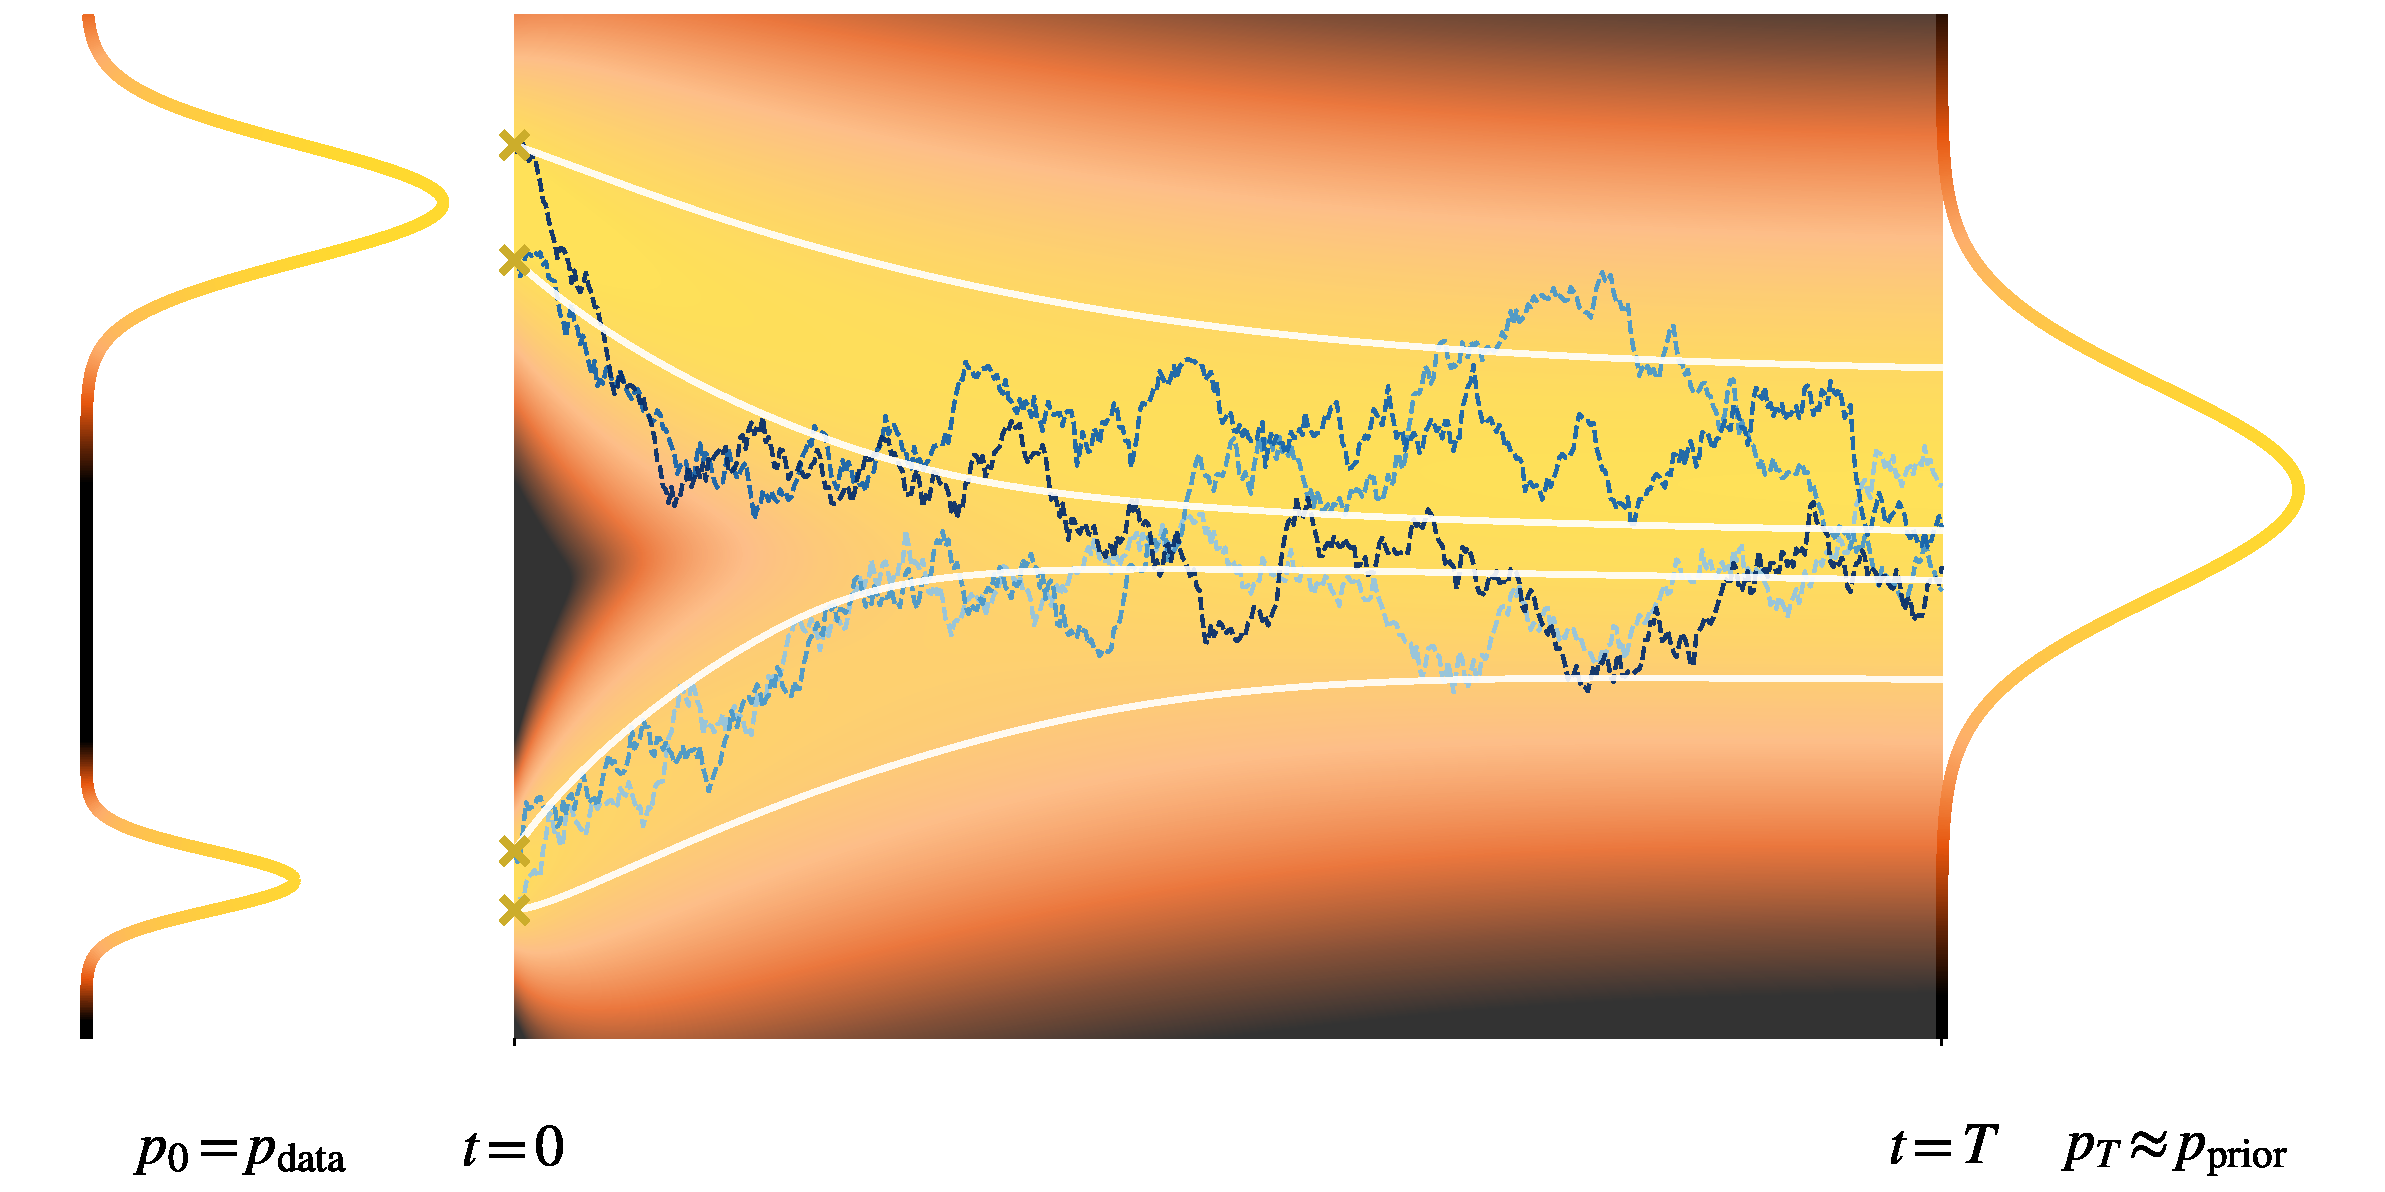
\includegraphics[width=\textwidth]{Images/PartB/forward_sde_ode_trajectories.pdf}
        \caption{\textbfs{(1D) Visualization of the forward process in a diffusion model.} The process starts from initial points sampled (denoted as ``$\times$'') from a  complex bimodal data distribution ($p_0 = p_{\mathrm{data}}$) and evolves toward a simple, unimodal Gaussian prior ($p_T \approx p_{\mathrm{prior}}$). The background heatmap illustrates the evolving marginal probability density, $p_t$, which smooths over time. Sample trajectories are shown evolving from $t=0$ to $t=T$, comparing the stochastic forward SDE process (blue paths) with its deterministic counterpart, the PF-ODE (white paths). Note that the PF-ODE is a deterministic transport map for densities, not generally the mean of sample paths started from a single point. \figcredit{Created by the authors.}}

    \label{fig:sde-density-traj}
\end{figure}


With this formulation, earlier methods based on discrete time, such as NCSN~\citep{song2019generative} and DDPM~\citep{sohl2015deep,ho2020denoising}, can be unified under the \emph{continuous-time} framework through a stochastic process $\rvx(t)$ governed by a forward SDE defined on the interval $[0, T]$:
\begin{mdframed}
\begin{equation}\label{eq:sde_forward}
    \diff\rvx(t) = \mathbf{f}(\rvx(t), t) \diff t + g(t) \diff\rvw(t), \quad \rvx(0) \sim p_{\mathrm{data}}.
\end{equation}
\end{mdframed}
Here, $\mathbf{f}(\cdot, t)\colon\mathbb{R}^D\to\mathbb{R}^D$ is the drift, $g(t) \in \mathbb{R}$ is the scalar diffusion coefficient, and $\rvw(t)$ denotes a standard Wiener process. We refer to this as the \emph{forward SDE}, which describes how clean data is gradually perturbed into noise over time.

Once the drift $\mathbf{f}$ and diffusion coefficient $g$ are specified, the forward process is fully determined, describing how the data variable is progressively corrupted through the injection of Gaussian noise. In particular, two families of time-dependent densities are induced:
\paragraph{Perturbation Kernels.} 
The conditional law
\[
p_t(\rvx_t |\rvx_0)
\]
describes how a clean data sample $ \rvx_0 \sim p_{\mathrm{data}} $ evolves into its noisy counterpart $\rvx_t$ at time $t$. In general, the drift term $\rvf(\rvx,t)$ in \Cref{eq:sde_forward} can be an arbitrary function of $\rvx$, but a common and analytically convenient choice is to assume it is affine:
\begin{equation}\label{eq:affine-drift}
    \rvf(\rvx,t) = f(t) \rvx, 
\end{equation}
where $f(t)$ is a scalar function of $t$, typically taken to be non-positive. 
Under this structure, the process remains Gaussian at every time, and the conditional distribution admits a closed-form solution obtained by solving the associated mean–variance ODEs~\citep{sarkka2019applied} (see also \Cref{subsec:scoresde-perturbation-kernel}). {In particular,
\[
p_t(\rvx_t |\rvx_0) = \mathcal{N} \big(\rvx_t; \rvm(t), P(t)\mathbf I_D\big),
\]
with
\[
\rvm(t) = \exp \Big(\int_0^t f(u) \diff u\Big) \rvx_0,
\quad
P(t) = \int_0^t \exp \Big(2 \int_s^t f(u) \diff u\Big) g^2(s) \diff s,
\]
and initial conditions $\rvm(0)=\rvx_0$, $P(0)=0$.}

This explicit form allows one to sample $\rvx_t$ given $\rvx_0$ directly, without numerically integrating the SDE, hence the term \emph{simulation-free}. Both NCSN and DDPM fall into this affine-drift setting. 

In the remainder, we develop the general theory for arbitrary drifts $\rvf(\rvx,t)$, but will return to the affine drift when closed-form analysis is useful.



\paragraph{Marginal Densities.} 
The time-marginal density $ p_t(\rvx_t) $ is obtained by integrating over the perturbation kernel:
\begin{equation}\label{eq:scoresde-oracle-marginal}
    p_t(\rvx_t) := \int p_t(\rvx_t|\rvx_0) p_{\mathrm{data}}(\rvx_0) \diff \rvx_0, \quad \text{with } p_0 = p_{\mathrm{data}}.
\end{equation}

{By choosing the coefficients $f(t)$ and $g(t)$ appropriately, the forward process gradually adds noise until the influence of the initial state is effectively forgotten. As $T$ becomes large, the conditional distribution $p_T(\mathbf{x}_T |\mathbf{x}_0)$ no longer depends on $\mathbf{x}_0$, because its mean evolves as
\[
\rvm(T) = \exp\!\Big(\int_0^T f(u)\diff u\Big) \mathbf{x}_0  \longrightarrow  \mathbf{0}, \quad \text{as } T\to\infty,
\]
provided $f(u)$ is non-positive so that the exponential factor decays. At the same time, the variance grows and stabilizes to match a chosen prior distribution.} Consequently, the marginal
\[
p_T(\mathbf{x}_T) = \int p_T(\mathbf{x}_T |\mathbf{x}_0) p_{\mathrm{data}}(\mathbf{x}_0)\diff\mathbf{x}_0,
\]
which initially represents a complicated mixture over data samples, converges to a simple prior $p_{\mathrm{prior}}$, typically Gaussian. In this limit,
\[
p_T(\mathbf{x}_T) \approx p_{\mathrm{prior}}(\mathbf{x}_T) 
\quad \text{and} \quad 
p_T(\mathbf{x}_T |\mathbf{x}_0) \approx p_{\mathrm{prior}}(\mathbf{x}_T),
\]
so the forward process maps any data distribution into a tractable prior, providing a convenient starting point for reversal and generation.







\subsection{Reverse-Time Stochastic Process for Generation}\label{subsec:reverse-sde}



\begin{figure}[th!]
    \centering
    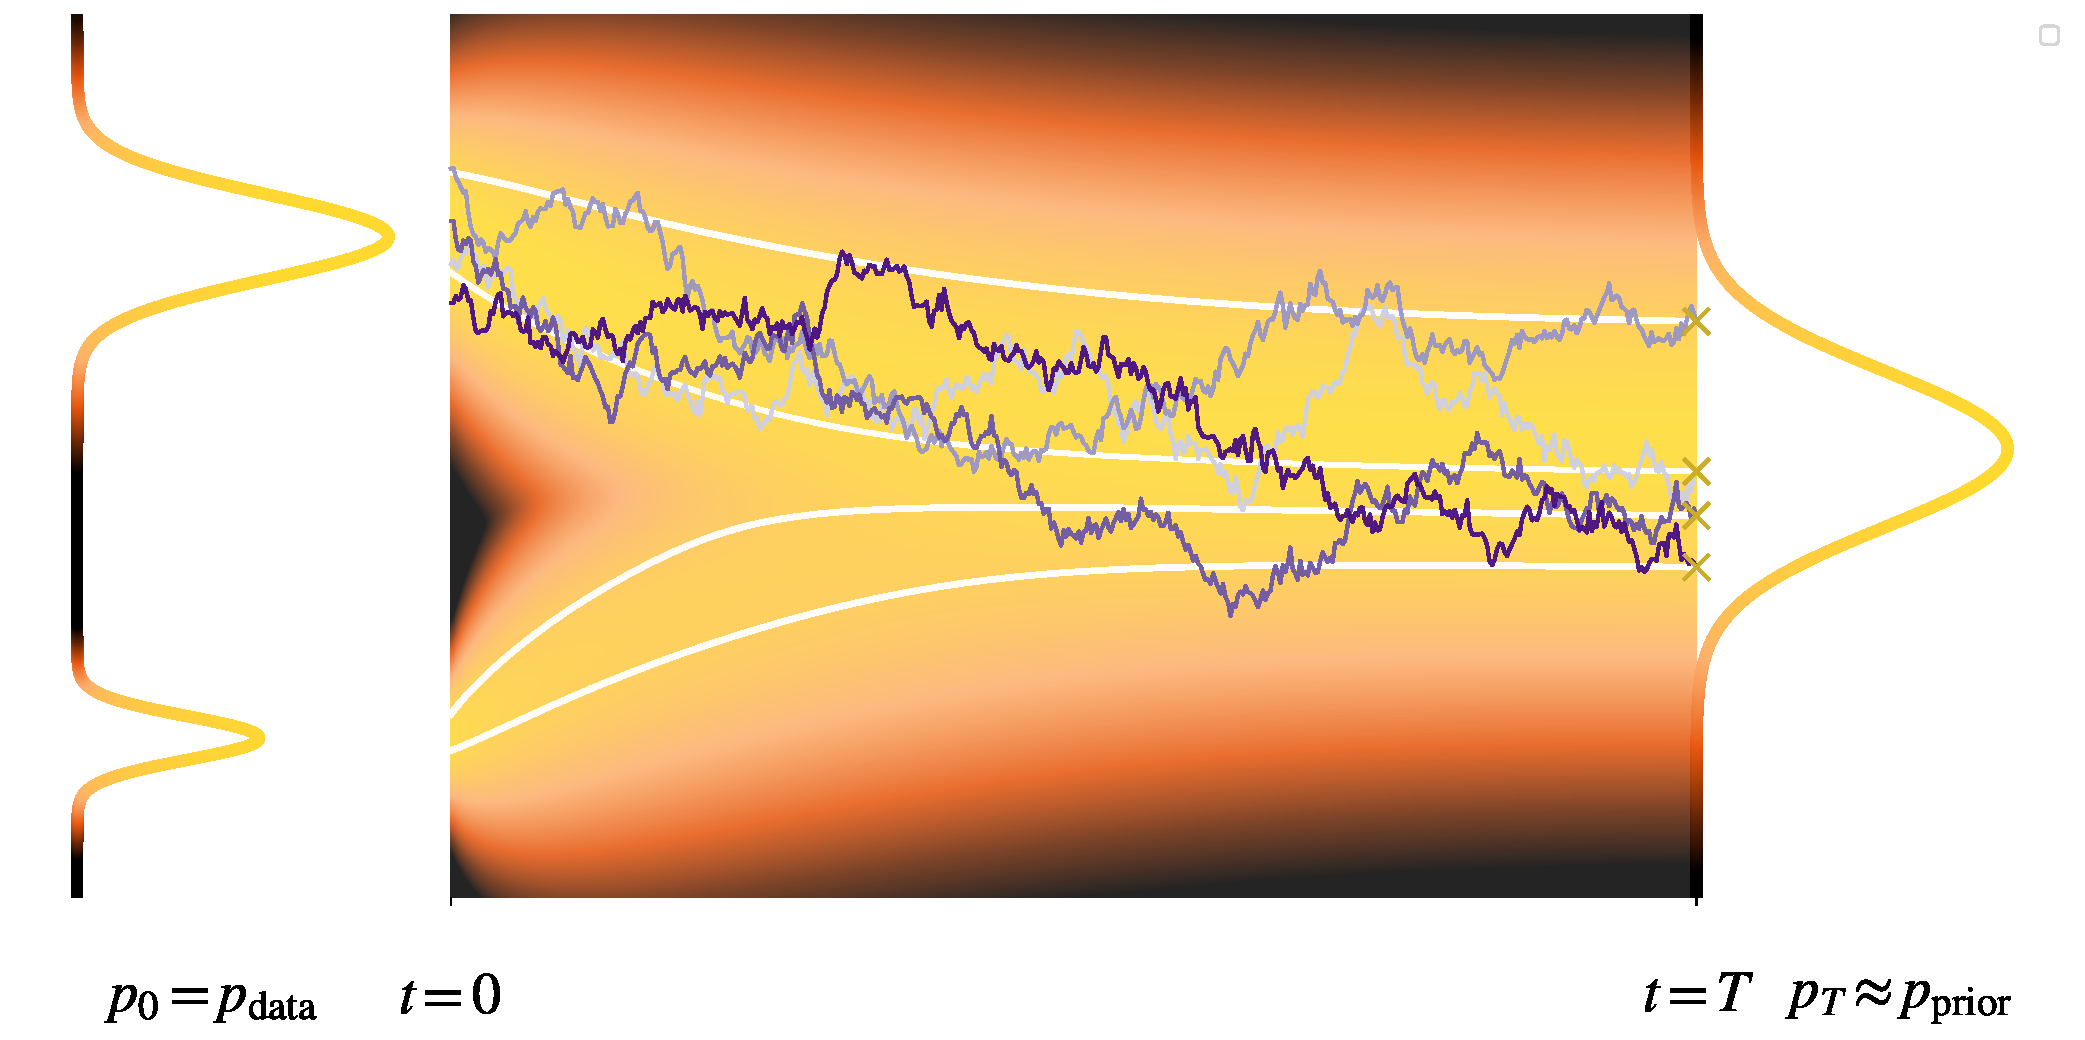
\includegraphics[width=\textwidth]{Images/PartB/reverse_sde_and_ode_trajectories.pdf}
    \caption{\textbfs{Visualization of the reverse-time stochastic process for data generation.} 
It begins from samples drawn from a simple prior distribution 
($p_{\mathrm{prior}}$) at $t=T$ (denoted as ``$\times$''), which are evolved backward 
in time using a reverse-SDE. The resulting trajectories terminate at $t=0$ 
and collectively form the target bimodal data distribution 
($p_0 = p_{\mathrm{data}}$). The background heatmap illustrates how the 
probability density is gradually transformed from a simple Gaussian into 
the complex target distribution.
\figcredit{Created by the authors.}}
    \label{fig:sde-density-back-traj}
\end{figure}
Intuitively, data generation from noise can be achieved by ``reversing'' the forward process: starting from a random point sampled from the prior distribution and evolving it backward in time to obtain a generated sample. For deterministic systems (that is, ODEs), this idea works naturally. Since no randomness is involved, reversing time simply means tracing the trajectory of a point in the opposite direction along the same path as in the forward process\footnote{Technically, this corresponds to solving the ODE with a time-flipping substitution $t \leftrightarrow T - t$.}. In contrast, SDEs incorporate stochasticity at every time step, meaning that a single point can evolve along many plausible random trajectories. As a result, reversing such processes is more subtle\footnote{Naively flipping time does not yield the correct reverse process.}. 

While individual stochastic trajectories are not reversible, the remarkable insight is that the distribution over these trajectories can be reversed. This is formalized by a foundational result from \citet{anderson1982reverse}, which shows that the time-reversed process $\{ \bar{\rvx}(t) \}_{t \in [0, T]}$\footnote{We use the ``bar'' notation to distinguish the reverse process $\{ \bar{\rvx}(t) \}_{t \in [0, T]}$ from the forward process $\{ \rvx(t) \}_{t \in [0, T]}$, defined by the forward-time SDE.} of the forward process in \Cref{eq:sde_forward} is itself governed by a well-defined SDE. This reverse-time process evolves from $T$ to $0$, and its dynamics are given by:
\begin{mdframed}
\begin{align}\label{eq:sde_backward}
\begin{aligned}[t]
    \diff\bar{\rvx}(t) = \left[\mathbf{f}(\bar{\rvx}(t), t) {\color{orange} - g^2(t) \nabla_{\rvx} \log p_t(\bar{\rvx}(t))} \right] \diff t + g(t) \diff \bar{\rvw}(t), \\
    \hfill\bar{\rvx}(T) \sim p_{\mathrm{prior}} \approx p_T.
\end{aligned}
\end{align}
\end{mdframed}
Here, $\bar{\rvw}(t)$ denotes a standard Wiener process in reverse time, defined as $\bar{\rvw}(t) := \rvw(T - t) - \rvw(T)$.

To build intuition for \Cref{eq:sde_backward}, we present a concrete example in \Cref{subsec:example-gaussian} with a Gaussian data distribution and linear–Gaussian dynamics. This setting is analytically tractable: one can derive the time-reversal formula directly using basic calculus and linear algebra, without invoking the full general theory of \citet{anderson1982reverse}.
% \se{the gaussian linear dynamics system case could be instructive, you can work out the time reversal formula from basic math/linear algebra}

Note that the presence of stochasticity ($g\neq 0$) introduces an additional correction term, $ -g^2(t) \nabla_{\rvx} \log p_t(\bar{\rvx}(t))$, which accounts for the effect of diffusion and ensures that the reversed dynamics correctly reproduce the evolution of marginal distributions induced by the forward SDE (see \Cref{subsec:fpe-sde-ode}).

\paragraph{Conceptually, Why Does the Reverse Process Work?} \Cref{subsec:reverse-sde-reason} presents an intuitive derivation of the reverse-time SDE by connecting it to the DDPM variational framework (optional but insightful). Here, we provide complementary intuition for how the reverse-time dynamics recover structured data from noise. 


At first glance, the presence of Brownian noise in the reverse time process may seem paradoxical. If the forward diffusion spreads data into increasingly noisy configurations, it is unclear how reversing this process, particularly one that introduces additional randomness through $\bar{\rvw}(t)$, can produce clean, structured samples concentrated near the data manifold. The key point is that the reverse time SDE does not inject arbitrary randomness. The diffusion term $g(t)\diff\bar{\rvw}(t)$ is always coupled with the score–driven drift $- g^2(t)\nabla_{\rvx}\log p_t(\bar{\rvx}(t))$. Together, these terms balance one another: the score guides trajectories toward regions of higher density, while the noise introduces controlled stochasticity that allows exploration without overwhelming the dynamics.
% \se{refer to langevin?} 

To see this more clearly, return to the Langevin intuition in \Cref{eq:continuous-langevin}. When $f(t)\equiv 0$, \Cref{eq:sde_backward} reads
\[
\diff\bar{\rvx}(t)
= - g^2(t) \nabla_{\rvx}\log p_t\!\big(\bar{\rvx}(t)\big) \diff t
+ g(t)  \diff\bar{\rvw}(t).
\]
Reparameterize time forward via $s:=T-t$ (so $\diff t=-\diff s$), and rename the Brownian motion in law so that $\diff\bar{\rvw}(t)=-\diff\rvw_s$. Writing $\bar{\rvx}_s:=\bar{\rvx}(T-s)$ and $\pi_s:=p_{T-s}$ then gives
\begin{align*}
    \diff\bar{\rvx}_s
&= g^2(T-s) \nabla\log \pi_s \big(\bar{\rvx}_s\big) \diff s
+ g(T-s) \diff\rvw_s
\\&=
2\tau(s) \nabla\log \pi_s\!\big(\bar{\rvx}_s\big) \diff s
+ \sqrt{2\tau(s)} \diff\rvw_s,
\quad
\tau(s):=\tfrac{1}{2}g^2(T-s).
\end{align*}
This has the Langevin form with a time-varying temperature $\tau(s)$, targeting the evolving density $\pi_s$. By Tweedie's formula (\Cref{eq:tweedie}), the score direction $\nabla\log \pi_s$ points toward the conditional clean signal at each time slice, so the drift continually ``pulls back'' denoised structure.

Crucially, $g(t)$ is \emph{annealing} along the reverse trajectory. Early on ($s\approx 0$, i.e., $t\approx T$), $g(T-s)$ is typically larger, so the injected noise is stronger and the process explores broadly. As $s$ increases, $g(T-s)$ decreases, the stochastic term weakens, and the score term dominates, pulling samples into high-density regions of $\pi_s$; by $s=T$ (i.e., $t=0$), trajectories concentrate near the data manifold.



% \se{refer to langevin?}

\paragraph{Overview of Reverse-Time SDE Capabilities.}

% \se{i think it's worth saying that solving the reversesde generates sampling, and it's completely determined by the scores (so if we know them, we have all we need)}
It is fascinating how the time-dependent score function
\[
\rvs(\rvx, t) := \nabla_{\rvx} \log p_t(\rvx)
\]
naturally appears in \Cref{eq:sde_backward}. Once the forward coefficients $f(t)$ and $g(t)$ are specified, the score is the only remaining unknown in the reverse dynamics. This highlights its central role: with the score in hand, the reverse process is determined, and sampling amounts to numerically integrating \Cref{eq:sde_backward} with the learned score.

Since the oracle score generally lacks a closed-form expression, we adopt the approach of \Cref{ch:score-based} and train a neural network $\mathbf{s}_{\bm{\phi}}(\rvx, t)$ to approximate it via score matching; see \Cref{subsec:sde-train} for details. Substituting $\rvs(\rvx, t)$ with $\mathbf{s}_{\bm{\phi}}(\rvx, t)$ in \Cref{eq:sde_backward} then specifies the reverse dynamics completely.

Generation corresponds to solving the reverse-time SDE reversely from $t = T$, starting with $\rvx_T \sim p_{\mathrm{prior}}$, to $t = 0$. Importantly, \citet{anderson1982reverse} proves that the marginal densities of the forward and reverse processes coincide, ensuring that samples at $t=0$ approximately follow $p_{\mathrm{data}}$ when $p_{\mathrm{prior}} \approx p_T$. We will explore this further in \Cref{subsec:sde-sample}.






\subsection{Deterministic Process (Probability Flow ODE)  for Generation}\label{subsec:pf-ode}
 Although the SDE in \Cref{eq:sde_backward} introduces stochasticity and potentially increases the diversity of generated samples, a question arises:
\begin{question}
    Is it necessary to sample using the SDE in \Cref{eq:sde_backward}?
\end{question}

Inspired by \citet{maoutsa2020interacting}, \citet{song2020score} also introduced a deterministic process, an ODE, that evolves samples with the same marginal distributions as the forward SDE. This process $\{\tilde\rvx(t)\}_{t\in[0,T]}$\footnote{We use a tilde to distinguish processes associated with the forward and reverse-time SDEs. Going forward, we omit this notational distinction for simplicity.}, called the \emph{Probability Flow ODE (PF-ODE)}, is given by:
\begin{mdframed}
    \begin{equation}\label{eq:prob_ode_gt}
    \frac{\diff}{\diff t}\tilde\rvx(t) = \mathbf{f}(\tilde\rvx(t), t) - \frac{1}{2} g^2(t) \nabla_{\rvx} \log p_t(\tilde\rvx(t)).
    \end{equation}
\end{mdframed}

Analogous to the SDE case, one can replace the true score with a learned approximation and integrate the reverse-time ODE from $t = T$ to $t = 0$ to generate samples. Concretely, the generated sample (solution of PF-ODE at time $t=0$) takes the form
\[
\tilde\rvx(T) + \int_{T}^{0} \Big[ \mathbf{f}(\tilde\rvx(\tau), \tau) - \frac{1}{2} g^2(\tau)  \nabla_{\rvx} \log p_\tau(\tilde\rvx(\tau)) \Big]   \diff \tau,
\]
where the initial condition $\tilde\rvx(T) \sim p_{\mathrm{prior}}$. Since this integral is intractable in closed form, practical generation relies on numerical solvers (e.g., Euler method, see \Cref{eq:euler-maruyama}).

Compared to the reverse-time SDE, the PF-ODE offers two key advantages:
\begin{itemize}
    \item The ODE can be integrated in either direction, from $t=0$ to $t=T$ or from $t=T$ to $t=0$, using the same formulation of the equation, provided the corresponding initial condition is specified at the chosen endpoint. This bidirectionality contrasts with SDEs, which generally admit only forward time integration.
    \item It benefits from a wide range of well-established, off-the-shelf numerical solvers developed for ODEs.
\end{itemize}


We emphasize that the PF-ODE is not obtained by simply removing the diffusion term in \Cref{eq:sde_backward}; notably, the factor of $\frac{1}{2}$ in its drift term has a principled origin. At a high level, \Cref{eq:prob_ode_gt} arises by choosing the drift of an ODE such that its evolution preserves the same marginal densities as the forward SDE in \Cref{eq:sde_forward}. The underlying principle (i.e., Fokker-Planck Equation~\citep{oksendal2003stochastic}) ensuring this alignment of marginals will be detailed in the next section.


\clearpage
\newpage



\section{Matching Marginals in Forward/Reverse-Time SDEs and PF-ODE}\label{subsec:fpe-sde-ode}
\begin{figure}[th!]
% \vspace{-0.1cm}
    \centering
    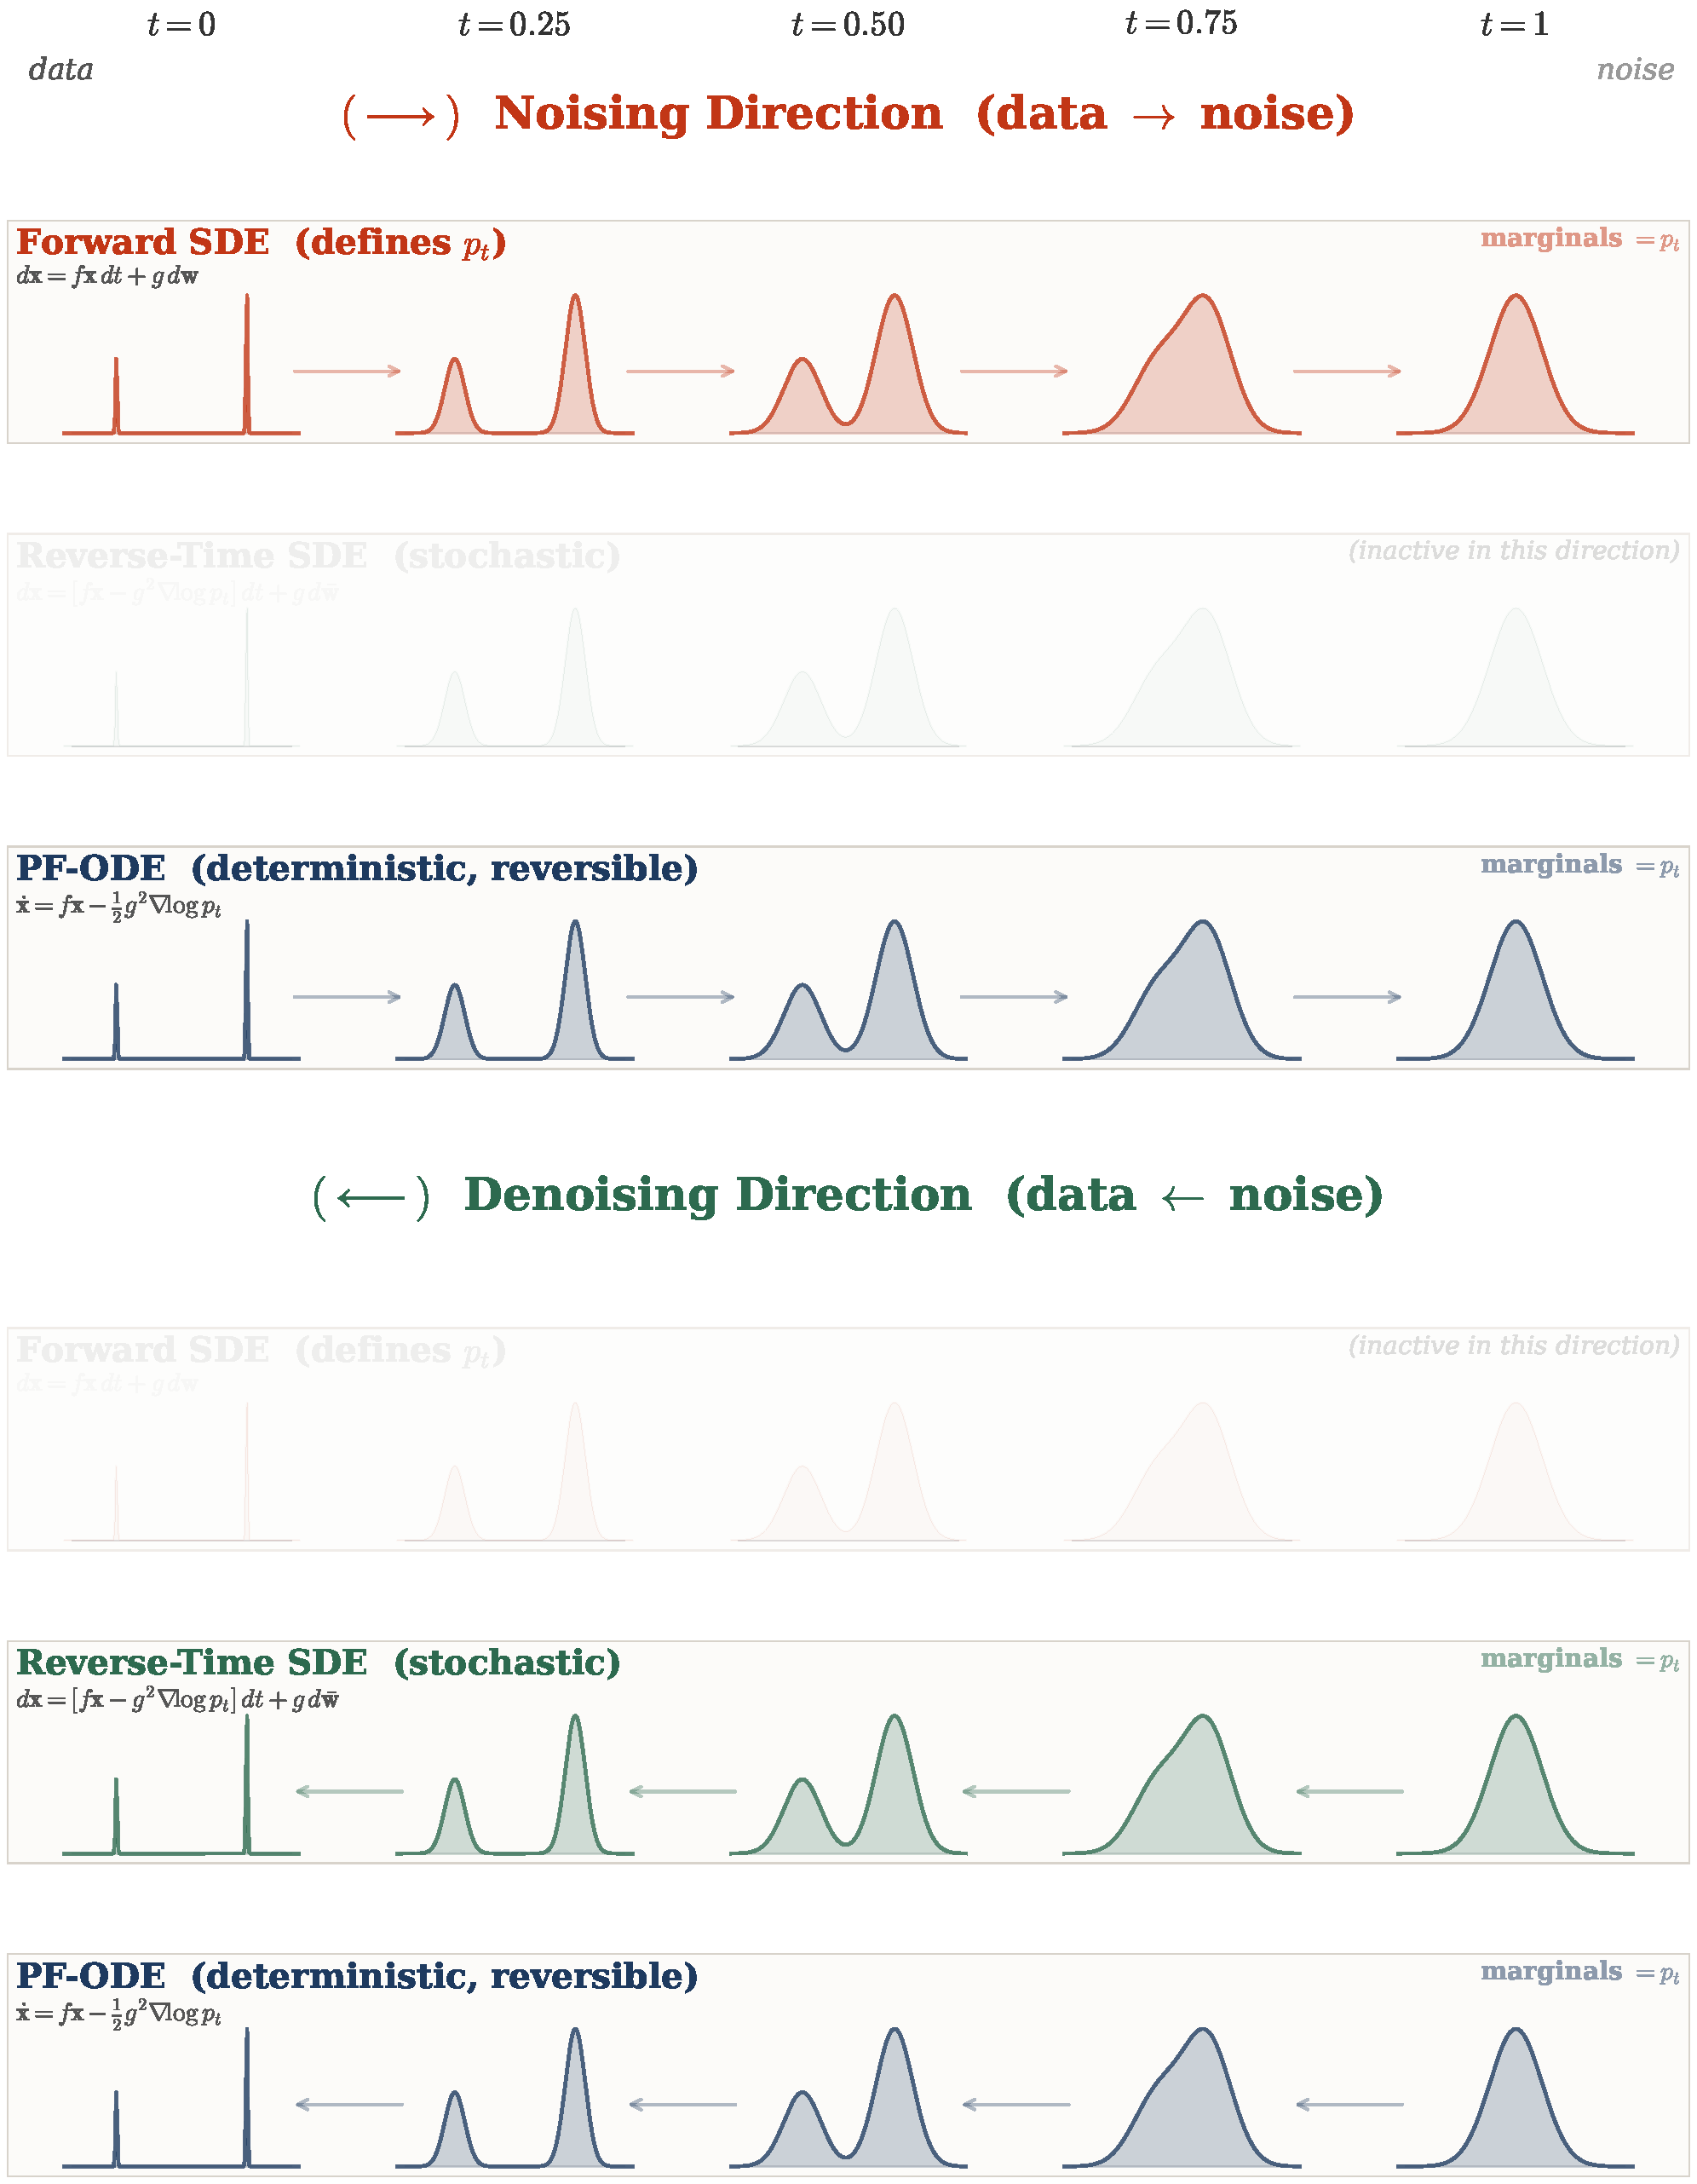
\includegraphics[width=\linewidth]{Images/PartB/score_sde_three_dynamics.pdf}
\caption{\textbfs{Three dynamics sharing the same marginals $p_t$.}
The forward SDE, which serves as an anchor reference, defines the marginals $p_t$ by diffusing data toward a Gaussian prior.
The reverse-time SDE and the PF-ODE yield the same marginals, as guaranteed by the Fokker-Planck equation, while moving in the denoising direction through the score $\nabla \log p_t$.
The top panel shows noising, given by the forward SDE or, equivalently at the marginal level, the PF-ODE run forward in time.
The bottom panel shows denoising, given by the reverse-time SDE or the PF-ODE run backward in time.
The PF-ODE appears in both panels because it is deterministic and time-reversible.
\figcredit{Created by the authors with AI-assisted coding.}}
    \label{fig:score-sde-three-dynamics}
    \vspace{-2cm}
\end{figure}
In this section, we present the \emph{Fokker-Planck equation} as the central principle governing diffusion models. It describes how probability densities evolve under noisy dynamics and serves as the natural analogue of a change-of-variables formula when randomness is present (see \Cref{app:continuity}). Starting from the forward diffusion process, which defines the marginals $p_t$, we explain how both the reverse-time SDE and the PF-ODE are designed to reproduce the same marginal family. We then make this principle concrete through a Gaussian example, where the reverse-time SDE and the PF-ODE can be computed directly and explicitly.




% \begin{center}
% % \vspace{-0.2cm}
% \includegraphics[width=0.67\linewidth]{Images/PartB/density_evolution_3d_orange.pdf}
%     \captionof{figure}{\textbfs{(2D) Temporal evolution of the marginal density $p_t$.} The forward SDE has $\mathbf{f} \equiv \mathbf{0}$ and $g(t) = \sqrt{2t}$ on $[0,T]$. It starts with $p_0 = p_{\mathrm{data}}$ a two-mode Gaussian mixture and ends at $p_T \approx p_{\mathrm{prior}} := \mathcal{N}(\mathbf{0}, T^2 \mathbf{I})$.  The temporal-spatial evolution of $p_t$ follows the Fokker-Planck equation.
% }
%     \label{fig:fpe-density}
% \end{center}
\subsection{Fokker-Planck Equation to Ensure Alignment of Marginal Densities}
A central concept in diffusion models is that \emph{different processes can lead to the same sequence of marginal distributions} (as we will illustrate later in this subsection).
 The objective is to construct a process that transforms $p_{\mathrm{prior}}$ into $p_{\mathrm{data}}$ by aligning the marginals across time, and in particular at $t=0$. The exact form of the process is secondary, provided it is tractable and admits efficient sampling. This naturally leads to a fundamental question:


\begin{question}
How can we ensure that different processes yield identical marginal distributions?
\end{question}



Returning to our setup, once the forward SDE is specified, it defines the evolution of marginal densities from $p_{\mathrm{data}}$ to $p_{\mathrm{prior}}$. The reverse-time SDE and PF-ODE are then constructed so that their trajectories yield marginal distributions that exactly match those of the forward process. The key to this correspondence lies in the Fokker–Planck equation, which governs how marginal densities evolve under diffusion processes. An illustration is provided in \Cref{fig:score-sde-three-dynamics}. The following theorem~\citep{anderson1982reverse,song2020score} establishes the foundation for this connection:
\thmp{Fokker–Planck Equation Ensures Marginals Alignment}{fpe}{Let $\{\rvx(t)\}_{t\in[0,T]}$ evolves with the forward SDE
\[
\diff \rvx(t) = \rvf(\rvx(t),t)\diff t + g(t)\diff \rvw(t),
\]
with initial condition $\rvx(0)\sim p_0 = p_{\mathrm{data}}$.  Then its marginal densities $p_t$ satisfy the Fokker–Planck equation
\begin{align}\label{eq:fp_general}
\begin{aligned}
    \partial_t p_t(\rvx)
    &= - \nabla_{\rvx} \cdot\bigl[\rvf(\rvx,t) p_t(\rvx)\bigr]
       + \tfrac12 g^2(t) \Delta_{\rvx} p_t(\rvx)\\
    &= - \nabla_{\rvx} \cdot\bigl[\rvv(\rvx,t) p_t(\rvx)\bigr],
\end{aligned}
\end{align}
where $\Delta_{\rvx}$ denotes the Laplacian operator, and
\[
 \rvv(\rvx,t)
:= \rvf(\rvx,t)
  -\tfrac12 g^2(t) \nabla_{\rvx}\log p_t(\rvx).
\]
Then, both the PF‑ODE and the reverse‑time SDE yield the same family $\{p_t\}_{t \in [0, T]}$, with the latter evolving in reverse time:
\begin{enumerate}
  \item[\textup{(i)}] The \emph{PF‑ODE} $\{\tilde\rvx(t)\}_{t\in[0,T]}$
  \[
    \frac{\diff \tilde\rvx(t)}{\diff t}
    = \rvv(\tilde\rvx(t),t),
  \]
  if started with $\tilde\rvx(0)\sim p_0$ and run forward in $t$, or equivalently started with $\tilde\rvx(T)\sim p_T$ and run backward in $t$, has marginals $\tilde\rvx(t)\sim p_t$ for all $t\in[0,T]$.

  \item[\textup{(ii)}] The \emph{reverse‑time SDE} $\{\bar\rvx(t)\}_{t\in[0,T]}$
  \[
    \diff \bar\rvx(t)
    = \bigl[\rvf(\bar\rvx(t),t) - g^2(t)\nabla_{\rvx}\log p_t(\bar\rvx(t))\bigr]\diff t
      + g(t)\diff \bar\rvw(t),
  \]
  with $\bar\rvx(0)\sim p_T$ and $\bar\rvw(t)$ a standard Wiener process in reverse time, has marginals $\bar\rvx(t)\sim p_{T-t}$.
\end{enumerate}
}{The proof is provided in \Cref{app-sec:scoresde-fpe-proof}, while \Cref{subsec:fpe-reason} offers further intuition behind the Fokker–Planck equation using the marginalization technique of probability. 
% \se{fix language}
}


% \rmkb{Anderson's reverse-time SDE theorem enables reversing diffusion processes under conditions where the evolved densities $p_t$ are \emph{absolutely continuous w.r.t. Lebesgue measure}, smooth, and positive for $t > 0$, even if the initial data distribution $p_0 = p_{\mathrm{data}}$ is singular (e.g., supported on a lower-dimensional manifold, violating absolute continuity at $t=0$). The forward diffusion induces absolute continuity and smoothness for $t > 0$, allowing the score function $\nabla \log p_t$ to be defined. However, in practice for both the reverse SDE and the PF-ODE, integration backward stops at a sufficiently small $\varepsilon > 0$ rather than $t=0$ to avoid divergence of the score near $t=0$, where $p_t$ approaches singularity under the manifold hypothesis; this ensures numerical stability and sample quality on $(\varepsilon, T]$.

% For simplicity, we still write $t=0$ in our discussion, without explicitly denoting $t=\varepsilon$ as the stopping time.}
% \se{not sure this remark is particularly insightful}


\paragraph{Multiple Conditional Distributions for a Fixed Marginal.}
To understand how the PF-ODE transports $p_{\mathrm{data}}$ forward in time (or equivalently $p_{\mathrm{prior}}$ in reverse), consider the \emph{flow map} $\bPsi_{s \to t}: \mathbb{R}^D \to \mathbb{R}^D$, where $\bPsi_{s \to t}(\rvx_s)$ denotes the PF-ODE solution at time $t$ initialized from $\rvx_s$ at time $s$, for any time $s, t \in[0,T]$. In other words, this map takes an initial state $\rvx_s$ and directly jumps to its state at $t$:
\begin{align}\label{eq:flow-map-def}
\bPsi_{s \to t}(\rvx_s) \coloneqq \rvx_s + \int_s^t \rvv(\rvx_\tau, \tau)\mathrm{d}\tau,
\end{align}
with velocity field
\begin{align*}
\rvv(\rvx, \tau) := \rvf(\rvx, \tau) - \frac{1}{2} g^2(\tau)\nabla_{\rvx}\log p_\tau(\rvx).
\end{align*}
Here, the integral captures the net displacement accumulated along the PF-ODE trajectory $\rvx_\tau$. Under mild smoothness assumptions on $\rvv$, the flow map $\bPsi_{s \to t}: \mathbb{R}^D \to \mathbb{R}^D$ is a smooth bijection\footnote{Spoiler: the PF-ODE flow map $\bPsi_{s\to t}$ is exactly the Normalizing Flow (NF) bijection carrying $p_s$ to $p_t$ (to be detailed in \Cref{sec:flow-based-method}). The difference is that PF-ODE fixes the unique vector field dictated by the SDE’s Fokker–Planck dynamics, whereas NF (or continuous-time NF) parameterizes this field but relies on the same change-of-variables principle.
}.




For any $t\in[0,T]$, the \emph{pushforward density} is defined as
\[
p_t^{\mathrm{fwd}}(\rvx_t) := \int \delta\bigl(\rvx_t - \bPsi_{0 \to t}(\rvx_0)\bigr)\, p_{\mathrm{data}}(\rvx_0) \,\diff \rvx_0,
\]
denoted $\bm{\Psi}_{0\to t} \sharp p_{\mathrm{data}}$, representing the distribution at time $t$ under $\bm{\Psi}_{0\to t}$. Theorem~\ref{thm:fpe} ensures $p_t^{\mathrm{fwd}} = p_t$, where $p_t$ is the marginal density of the forward SDE, equating the deterministic PF-ODE and stochastic kernel:
\[
p_t(\rvx_t) = \int p_t(\rvx_t |\rvx_0)\, p_{\mathrm{data}}(\rvx_0)\,\diff \rvx_0
= \int \delta\bigl(\rvx_t - \bm{\Psi}_{0\to t}(\rvx_0)\bigr)\, p_{\mathrm{data}}(\rvx_0)\,\diff \rvx_0.
\]

This implies infinitely many conditionals $Q_t(\rvx_t |\rvx_0)$ yield the same $p_t(\rvx_t)$, for instance:
\begin{itemize}
  \item \textbfs{Stochastic (Simulation-Free):} $Q_t(\rvx_t |\rvx_0) = p_t(\rvx_t |\rvx_0)$,
  \item \textbfs{Deterministic (Requires ODE Solving):} $Q_t(\rvx_t |\rvx_0) = \delta\bigl(\rvx_t - \bm{\Psi}_{0\to t}(\rvx_0)\bigr)$,
  \item \textbfs{Mixture:} $Q_t(\rvx_t |\rvx_0) = \lambda p_t(\rvx_t |\rvx_0) + (1-\lambda)\delta\bigl(\rvx_t - \bm{\Psi}_{0\to t}(\rvx_0)\bigr)$, $\lambda\in[0,1]$.
\end{itemize}
This nonuniqueness of $Q_t(\rvx_t |\rvx_0)$ arises from the fact that the marginal constraint does not uniquely determine the conditional distribution. This concept reappears in \Cref{subsec:fm-framework} and \Cref{subsec:ddim}. In particular, there exists an entire family of reverse-time SDEs that are consistent with the same marginal $p_t$.

\msg{Observation}{Matching Prescribed Marginal Densities}{
Multiple processes can give rise to the same sequence of marginal densities; what truly matters is satisfying the Fokker–Planck equation. This fundamental insight affords us remarkable flexibility in designing generative processes that transition from $ p_{\mathrm{prior}} $ to $ p_{\mathrm{data}} $, or vice versa.
}
The Fokker–Planck equation lies at the heart of diffusion models and is rooted in the fundamental \emph{change-of-variable formula} for probability densities (see \Cref{app:continuity} for a systematic treatment). Far from being a minor technical detail, this principle recurs throughout our development, most notably in \Cref{sec:flow-matching-framework}.
% , and reveals deep structural connections among seemingly different formulations.
% \se{either cut or provide more detail here on this connection}



\subsection{A Computable Example: Evolutions of Gaussian Dynamics}\label{subsec:example-gaussian}
When $p_{\mathrm{data}}$ is a normal distribution (or a mixture of Gaussians), the score function admits a closed-form expression. 
This makes it an ideal setting for building intuition about diffusion processes: we can explicitly derive the reverse-time SDE and the PF-ODE using only basic calculus, without resorting to advanced mathematical tools. 
In this subsection, we illustrate how these equations behave in such a tractable case.



\paragraph{Exact Computation of the Reverse-Time SDE with a Gaussian.}
 When $p_{\mathrm{data}}$ is Gaussian, the formula in \Cref{eq:sde_backward} can be derived directly, without relying on the general theory and proofs of \citet{anderson1982reverse}. To illustrate the core idea, we consider the one-dimensional case; the extension to higher dimensions follows in the same way.

 


Start from the forward SDE
\[
\diff x(t)  =  f(t)  x(t)  \diff t  +  g(t)  \diff w_t,
\]
and take one small Euler step of size $\Delta t>0$:
\[
x_{t+\Delta t}  =  a  x_t  +  r  \epsilon,
\]
where $a:=1+f(t)\Delta t$, $r:=g(t)\sqrt{\Delta t}$, and $ \epsilon\sim\mathcal N(0,1)$. Equivalently, the forward one-step transition kernel is Gaussian:
\[
x_{t+\Delta t}   |   x_t  \sim  \mathcal N\!\big(a  x_t,   r^2\big).
\]
Since $p_{\mathrm{data}}$ is assumed to be Gaussian, the current marginal at time $t$ is also Gaussian, which takes the following form:
\[
x_t \sim \mathcal N(m_t,   s_t^2),
\]
for some scalar $m_t$ and $s_t$. So conditioning will amount to multiplying two Gaussians and renormalizing. This keeps the algebra elementary.

By Bayes’ rule the conditional density is, up to a constant, the product of the prior and the transition kernel:
\begin{align*}
    p(x_t   |   x_{t+\Delta t})  &\propto p(x_{t+\Delta t} | x_t   ) p_t(\rvx_t) \\&\propto
\exp\Big(-\frac{(x_t-m_t)^2}{2s_t^2}\Big)  
\exp\Big(-\frac{(x_{t+\Delta t}-a  x_t)^2}{2r^2}\Big).
\end{align*}
The exponent is a quadratic in $x_t$. Expanding both squares and grouping terms shows exactly which coefficients matter:
\[
-2\log p(x_t   |   x_{t+\Delta t})
 = 
A  x_t^2  -  2 B  x_t  +  \text{const},
\]
with
\[
A:=\frac{1}{s_t^2}+\frac{a^2}{r^2},\quad
B:=\frac{m_t}{s_t^2}+\frac{a  x_{t+\Delta t}}{r^2}.
\]
Here $A$ is the sum of precisions (prior precision plus the transition-kernel precision transported through $a$), while $B$ is the corresponding precision-weighted sum of targets. With these in hand, completing the square gives the posterior in one line:
\[
A x_t^2 - 2 B x_t
  =  
A\Big(x_t-\frac{B}{A}\Big)^2  -  \frac{B^2}{A},
\]
so the conditional distribution is Gaussian with variance $1/A$ and mean $B/A$:
\[
\Var(x_t   |   x_{t+\Delta t})   =   \frac{1}{\frac{1}{s_t^2}+\frac{a^2}{r^2}},
\qquad
\mathbb E[x_t   |   x_{t+\Delta t}]   =  
\frac{\frac{m_t}{s_t^2}+\frac{a  x_{t+\Delta t}}{r^2}}{\frac{1}{s_t^2}+\frac{a^2}{r^2}}.
\]
These closed forms already describe the reverse transition for any small $\Delta t$. To read off a reverse-time SDE, we now expand them for small $\Delta t$.

Use $a=1+f(t)\Delta t$ and $r^2=g^2(t)\Delta t$. As $\Delta t\to 0$, the contribution $\frac{a^2}{r^2}\sim \frac{1}{g^2(t)\Delta t}$ dominates the precision, so the variance becomes
\[
\Var(x_t   |   x_{t+\Delta t})
= \left(\frac{1}{s_t^2}+\frac{a^2}{r^2}\right)^{-1}
= g^2(t)  \Delta t  +  \mathcal{O}(\Delta t^2),
\]
which tells us the reverse step has the same diffusion scale $g(t)$ as the forward step. For the mean, expand the ratio $B/A$ to first order:
\[
\mathbb E[x_t   |   x_{t+\Delta t}]
  =  x_{t+\Delta t}
 +  \Delta t\left[
-\left(f(t)+\frac{g^2(t)}{s_t^2}\right)  x_{t+\Delta t}
 +  \frac{g^2(t)}{s_t^2}  m_t
\right]  +  \mathcal{O}(\Delta t^2).
\]

Putting the mean and variance together yields the one-step reverse transition kernel
\[
x_t    |    x_{t+\Delta t}
 \sim 
\mathcal N\!\left(
x_{t+\Delta t} + \Delta t\!\left[-\left(f+\frac{g^2}{s_t^2}\right)  x_{t+\Delta t} + \frac{g^2}{s_t^2}  m_t\right],
 g^2  \Delta t\right)
 +  \mathcal{O}(\Delta t^2).
\]
This is recognized as the Euler–Maruyama update, run backward from $t+\Delta t$ to $t$:
\[
x_t - x_{t+\Delta t}
= \Delta t\!\left[-\left(f+\frac{g^2}{s_t^2}\right) x_{t+\Delta t} + \frac{g^2}{s_t^2} m_t\right]
+ g\sqrt{\Delta t} \epsilon + O(\Delta t^2).
\]
Letting $\Delta t\to 0$ gives the SDE on the original clock (time decreasing along the path)
\[
\diff x(t)
= \Big[-\Big(f(t)+\frac{g^2(t)}{s_t^2}\Big) x(t) + \frac{g^2(t)}{s_t^2} m_t\Big]\diff t
+ g(t) \diff \bar w_t .
\]
This drift can be written with the score because for a Gaussian marginal $p_t=\mathcal N(m_t,s_t^2)$,
\[
\partial_x \log p_t(x) = -\frac{x-m_t}{s_t^2}
 \Longrightarrow 
-\Big(f+\frac{g^2}{s_t^2}\Big) x + \frac{g^2}{s_t^2} m_t
= -f x + g^2 \partial_x\log p_t(x).
\]
To express the conventional \emph{forward-in-$t$} reverse-time parametrization, define the reversed process $\bar x(t):=x(T-t)$ (so that we now evolve forward in $t$). The time flip turns the drift into
\[
\diff \bar x(t)
= \Big[ f(t) \bar x(t)  -  g^2(t) \partial_x \log p_t(\bar x(t)) \Big]\diff t
+ g(t)\diff \bar w_t,
\]
where $\bar x(T)\sim p_{\mathrm{prior}}\approx p_T$. This is exactly the conventional reverse-time SDE. In vector form this matches the general \Cref{eq:sde_backward} with $\nabla_{\rvx}\log p_t$ in place of the 1D derivative.

\paragraph{Exact Computation of PF–ODE with a Gaussian.}
When the data distribution is assumed to be Gaussian, we can also directly derive the PF-ODE formula, avoiding heavy machinery such as the Fokker–Planck equation. In the end, we will see that the marginal densities of the PF-ODE coincide with those of both the forward SDE and the reverse-time SDE, providing a constructive verification of the Fokker–Planck theory to be discussed in \Cref{subsec:fpe-sde-ode}.


Assume $x_t\sim\mathcal N(m_t,s_t^2)$ at time $t$. A small deterministic step of size $\Delta t$ can be written as a smooth map
\[
x_{t+\Delta t}=\Phi_{t,\Delta t}(x_t)
= x_t + \Delta t v_t(x_t) + \mathcal{O}(\Delta t^2),
\]
which is simply the first–order Taylor expansion in $\Delta t$. Our goal is to see what form $v_t$ must take so that, whenever the input is Gaussian, the output remains Gaussian.

To this end, expand $v_t$ around the current mean $m_t$:
\[
v_t(x)=v_t(m_t)+v_t'(m_t)(x-m_t)+\tfrac12 v_t''(m_t)(x-m_t)^2+\cdots.
\]
Now set $y:=x_t-m_t$, so that $y\sim\mathcal N(0,s_t^2)$. Next, center the output by subtracting its mean (to first order in $\Delta t$):
\[
z:=x_{t+\Delta t}-\mathbb E[x_{t+\Delta t}]
= y + \Delta t\!\left(v_t'(m_t) y+\tfrac12 v_t''(m_t) (y^2-s_t^2)\right)+\mathcal{O}(\Delta t^2).
\]
At this point, recall that a Gaussian has zero skewness; in other words, its third centered moment is zero. Therefore, computing $\mathbb E[z^3]$ to first order and using
$\mathbb E[y]=0$, $\mathbb E[y^2]=s_t^2$, $\mathbb E[y^3]=0$, $\mathbb E[y^4]=3s_t^4$,
we obtain
\[
\mathbb E[z^3]
= 3 \Delta t\cdot \tfrac12 v_t''(m_t) \big(\mathbb E[y^4]-s_t^2\mathbb E[y^2]\big)+\mathcal{O}(\Delta t^2)
= 3 \Delta t v_t''(m_t) s_t^4+\mathcal{O}(\Delta t^2).
\]
For the output to stay Gaussian for all small $\Delta t$, this quantity must vanish at order $\Delta t$, which forces $v_t''(m_t)=0$. Repeating the same argument for higher derivatives rules out higher powers as well. Consequently, $v_t$ must be linear plus a shift:
\[
v_t(x)=a_t x+b_t.
\]
Plugging this back into the step gives
\[
x_{t+\Delta t}=(1+\alpha_t \Delta t) x_t+\beta_t \Delta t+\mathcal{O}(\Delta t^2),
\qquad
\alpha_t:=a_t,\ \ \beta_t:=b_t.
\]

We now push $x_t\sim\mathcal N(m_t,s_t^2)$ through this map and track mean and variance to first order:
\begin{align*}
\mathbb E[x_{t+\Delta t}]
&= m_t+\Delta t(\alpha_t m_t+\beta_t)+\mathcal{O}(\Delta t^2),
\\
\Var(x_{t+\Delta t})
&= s_t^2+\Delta t (2\alpha_t s_t^2)+\mathcal{O}(\Delta t^2).
\end{align*}
On the other hand, the forward SDE $\diff x=f(t) x \diff t+g(t) \diff w_t$ has the elementary moment formulas (see \Cref{eq:mean-var-evolution}):
\[
m_t' = f(t) m_t,
\qquad
(s_t^2)' = 2 f(t) s_t^2 + g^2(t).
\]
Matching the coefficients of $\Delta t$ gives
\[
\alpha_t = f(t)+\frac{g^2(t)}{2 s_t^2},
\qquad
\beta_t = - \frac{g^2(t)}{2 s_t^2} m_t.
\]

With these choices, the step becomes
\[
x_{t+\Delta t}
= x_t + \Delta t\!\left[\Big(f(t)+\frac{g^2(t)}{2s_t^2}\Big)x_t
-\frac{g^2(t)}{2s_t^2} m_t\right]+\mathcal{O}(\Delta t^2).
\]
Since for a Gaussian $p_t=\mathcal N(m_t,s_t^2)$ we have $\partial_x\log p_t(x)=-(x-m_t)/s_t^2$, we can rewrite the bracket as
$f(t) x_t - \tfrac12 g^2(t) \partial_x\log p_t(x_t)$.
Therefore,
\[
x_{t+\Delta t}
= x_t + \Delta t\Big[f(t) x_t - \tfrac12 g^2(t) \partial_x\log p_t(x_t)\Big] + \mathcal{O}(\Delta t^2).
\]
Finally, dividing by $\Delta t$ and letting $\Delta t\to 0$ yields the PF-ODE
\[
x'(t)  =  f(t) x(t)  -  \tfrac12 g^2(t) \partial_x\log p_t\!\big(x(t)\big).
\]

To see why this ODE has the same marginals as the forward SDE (and the reverse–time SDE), observe that the drift above is linear plus a shift. Thus $x(t)$ depends affinely on $x(0)$, and affine maps send Gaussians to Gaussians. Moreover, the mean $m_t$ and variance $s_t^2$ along this ODE satisfy exactly the same two scalar ODEs as the forward SDE (by our matching), with the same initial values. Hence $p_t=\mathcal N(m_t,s_t^2)$ is identical for both evolutions at every time $t$.





\clearpage
\newpage




\section{Score SDE: Its Training and Sampling}\label{sec:scoresde-training-sampling}

\subsection{Training}\label{subsec:sde-train}
Building on the philosophy as in \Cref{ch:score-based}, we approximate the oracle score $\nabla_{\rvx} \log p_t(\rvx)$ using a time-conditioned neural network 
\[
\mathbf{s}_{\bm{\phi}} = \mathbf{s}_{\bm{\phi}}(\rvx, t)
\]
across all $t\in[0,T]$, by minimizing a score-matching objective as in \Cref{eq:sm}:
\begin{equation*}
\mathcal{L}_{\text{SM}}(\bm{\phi}; \omega(\cdot)) := \frac{1}{2} \mathbb{E}_{t\sim p_{\text{time}}}  \mathbb{E}_{\rvx_t \sim p_t}\left[\omega(t) \left\|\mathbf{s}_{\bm{\phi}}(\rvx_t, t) - \nabla_{\rvx} \log p_t(\rvx_t)\right\|_2^2\right],
\end{equation*}
where $p_{\text{time}}$ is some time distribution (e.g., uniform on $[0,T]$), $\omega(\cdot)$ is a time-weighting function.

\begin{figure}[th!]
    \centering
    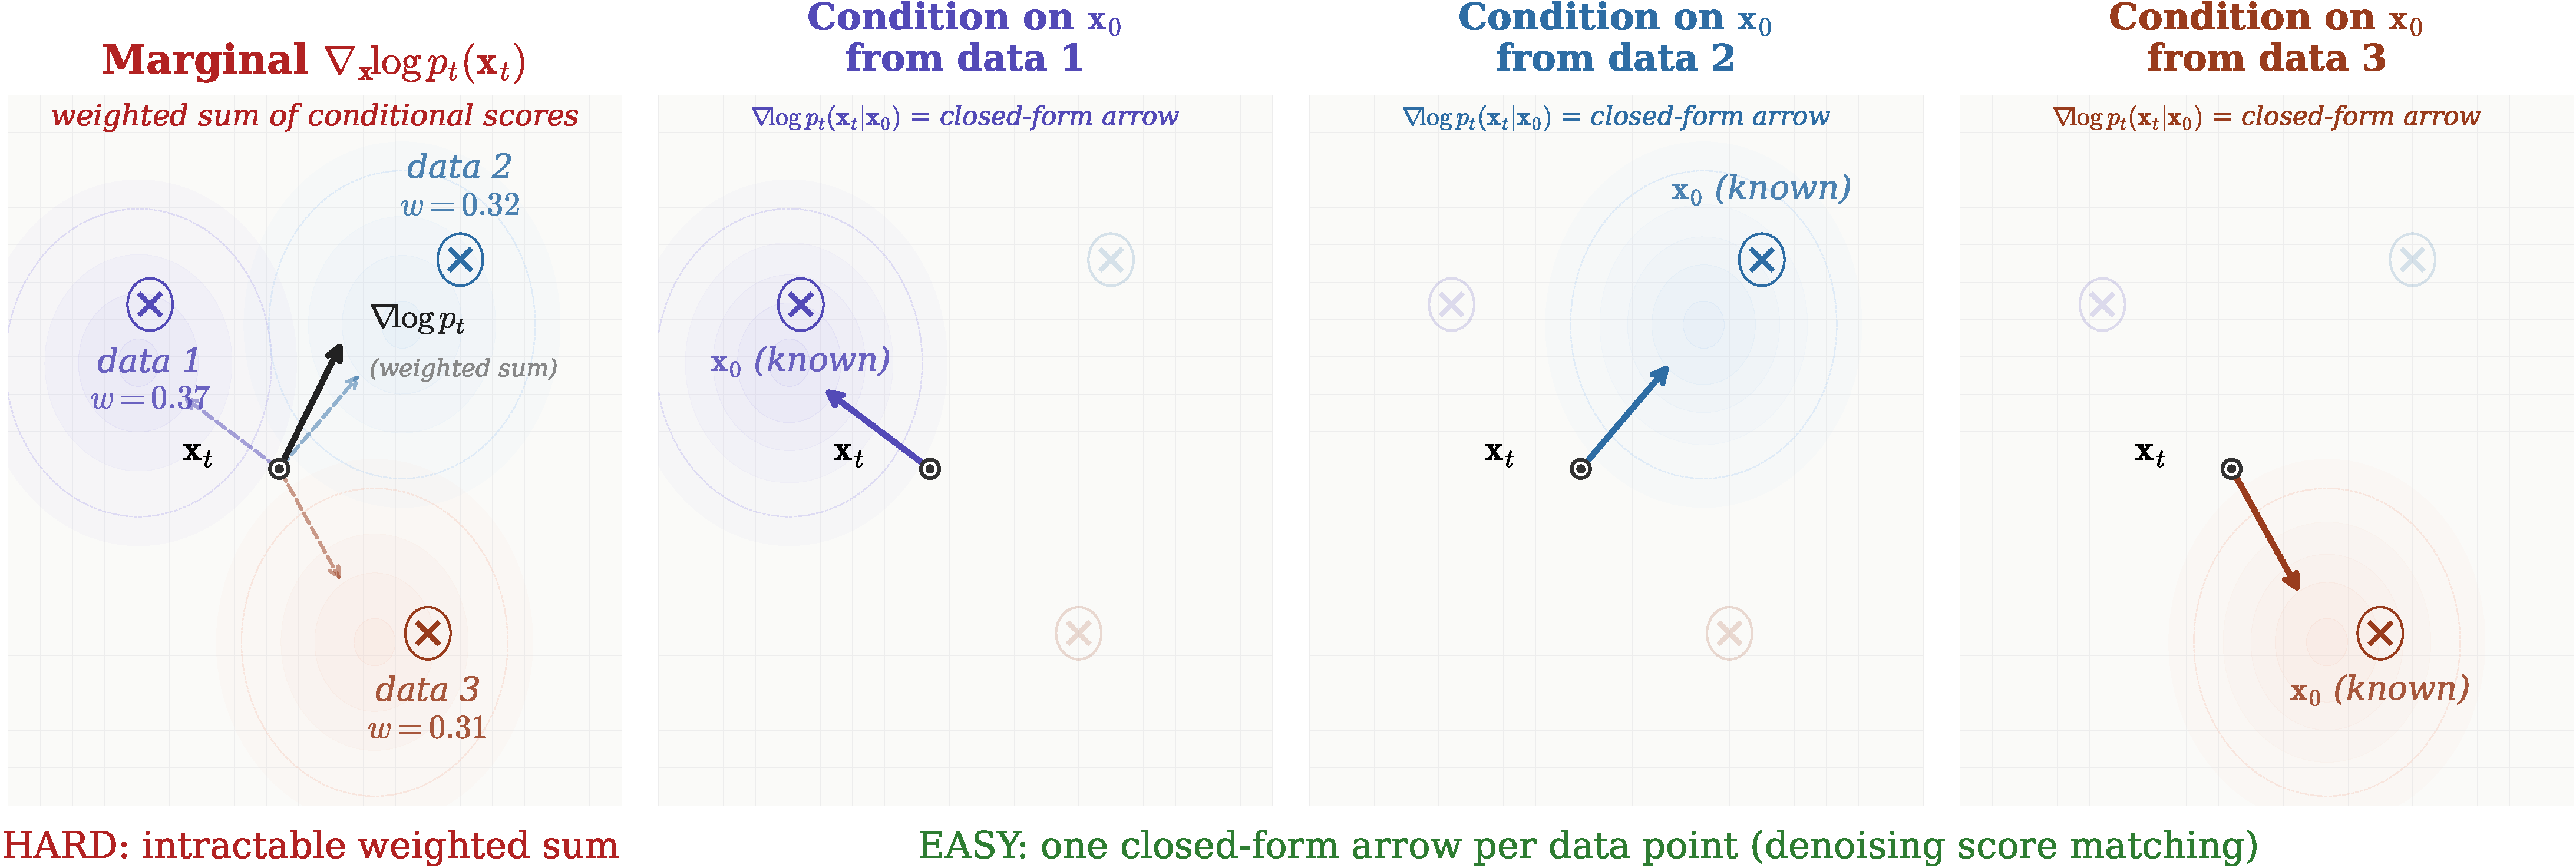
\includegraphics[width=\linewidth]{Images/PartB/denoising_score_matching.pdf}
    \caption{\textbfs{Illustration of the denoising score matching trick.}
The marginal score $\nabla_{\rvx_t}\log p_t(\rvx_t)$ is generally an intractable weighted average of the conditional scores over all possible clean samples $\rvx_0$, where the weights are given by the posterior distribution of $\rvx_0$ conditioned on the noisy observation $\rvx_t$.
However, for each fixed $\rvx_0$, the conditional score $\nabla_{\rvx_t}\log p_t(\rvx_t|\rvx_0)$ is available in closed form.
Denoising score matching turns this hard marginal estimation problem into an easy per-sample regression problem.
\figcredit{Created by the authors with AI-assisted coding.}}
    \label{fig:score-and-denoising-score}
\end{figure}


To avoid relying on the intractable oracle score $\nabla_{\rvx} \log p_t(\rvx)$, the DSM loss in \Cref{eq:dsm-loss} is employed. Conditioned on a data point $\rvx_0$, this approach allows the use of the analytically tractable score $\nabla_{\rvx_t} \log p_t(\rvx_t|\rvx_0)$ via \Cref{eq:score-gaussian-formula}, with concrete examples given in \Cref{sec:instances}. Specifically, we exploit the following loss function:
\begin{mdframed}
    \begin{equation}\label{eq:conti-dsm_loss-real}
\begin{aligned}
     &\mathcal{L}_{\text{DSM}}(\bm{\phi}; \omega(\cdot)) := \\
     &\frac{1}{2} \mathbb{E}_{t}  \mathbb{E}_{\rvx_0} \mathbb{E}_{ p_t(\rvx_t|\rvx_0)} \Big[\omega(t)\norm{\mathbf{s}_{\bm{\phi}}(\rvx_t, t) - \nabla_{\rvx_t} \log p_t(\rvx_t|\rvx_0)}_2^2 \Big],
\end{aligned}
\end{equation}
\end{mdframed}
where $\rvx_0 \sim p_{\mathrm{data}}$. \Cref{eq:conti-dsm_loss-real} can be interpreted as the continuous-time counterpart of \Cref{eq:nscn}, with the summation in the discrete case replaced by integration. 


Similar to the result in Theorem~\ref{thm:sm-dsm}, the minimizer of \Cref{eq:conti-dsm_loss-real} is uniquely determined as follows:

\proppp{Minimizer of DSM}{dsm-minimizer}{
The minimizer $\mathbf{s}^*$ satisfies
\begin{align}\label{eq:optimal-score}
\begin{aligned}
    \mathbf{s}^*(\rvx_t, t) 
    = \mathbb{E}_{\rvx_0 \sim p(\rvx_0 | \rvx_t)} \big[ \nabla_{\rvx_t} \log p_t(\rvx_t | \rvx_0) \big]= \nabla_{\rvx_t} \log p_t(\rvx_t),
\end{aligned}
\end{align}
for almost every $\rvx_t \sim p_t$ and $t \in [0,T]$. }{ 
DSM objective can be understood as a least-squares error problem. Specifically, at each time $t$, the optimal score function is given by the conditional expectation of the gradient of the log conditional density, which, under Bayes' rule, is equivalent to the gradient of the log marginal density. For a detailed proof, see Appendix~\ref{app-sec:min-dsm}.
}


\subsection{Sampling and Inference}\label{subsec:sde-sample}
\begin{figure}[th!]
    \centering
    \vspace{-0.8cm}
    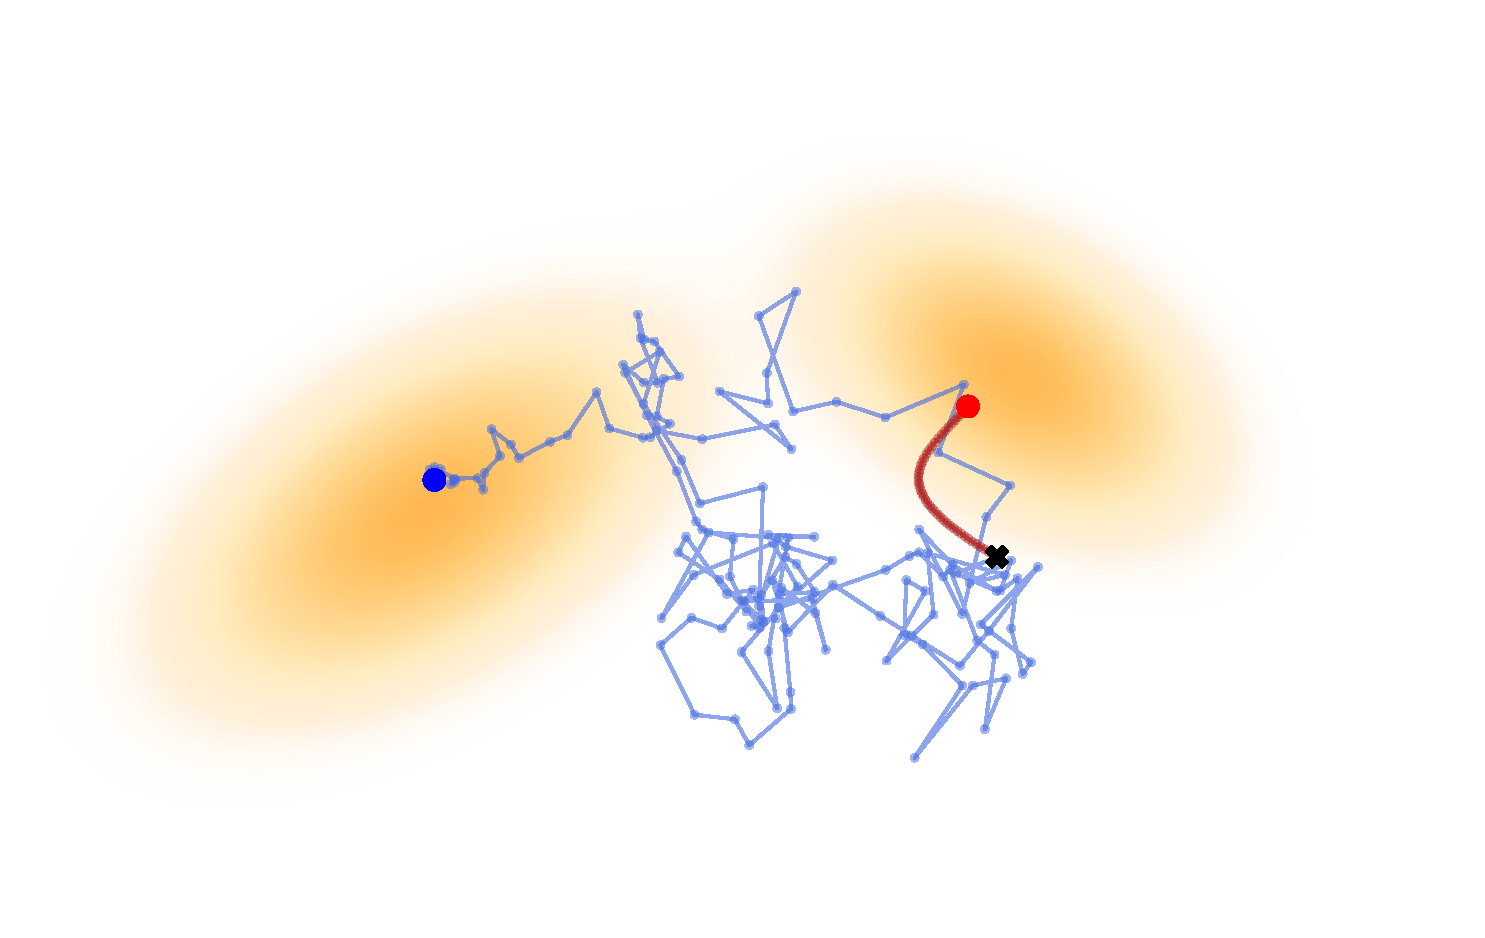
\includegraphics[width=\linewidth]{Images/PartB/sde_ode_trajectories.pdf}
    \vspace{-0.6cm}
    \caption{\textbfs{(2D) Illustration of sampling from the Score SDE.} The forward SDE is designed as $\diff\rvx(t)=\sqrt{2t}\diff\rvw(t)$, with drift $\mathbf{f}\equiv\mathbf{0}$ and diffusion coefficient $g(t)=\sqrt{2t}$ on $[0,T]$, evolves a two-mode Gaussian mixture $p_0=p_{\mathrm{data}}$ into $p_T\approx p_{\mathrm{prior}}:=\mathcal{N}(\mathbf{0},T^2\mathbf{I})$. Shown are sampling trajectories of the reverse-time SDE (blue; solved by \Cref{eq:euler-maruyama}) and the PF-ODE (red; solved by \Cref{eq:euler-ode}). Starting from a random point $\rvx_T\sim p_{\mathrm{prior}}$ (dark ``$\times$''), both trajectories move toward the support of $p_{\mathrm{data}}$ as $t\to 0$.
    \figcredit{Created by the authors.}}
    \label{fig:sde_ode_trajectories}
\end{figure}


After learning 
\[
\mathbf{s}_{\bm{\phi}^\times} := \mathbf{s}_{\bm{\phi}^\times}(\rvx, t) \approx \nabla_{\rvx} \log p_t(\rvx),
\]
we replace the intractable oracle score $\nabla_{\rvx} \log p_t(\rvx)$ in the reverse-time SDE (\Cref{eq:sde_backward}) and PF-ODE (\Cref{eq:prob_ode_gt}) with the learned proxy $\mathbf{s}_{\bm{\phi}^\times}(\rvx, t)$. This substitution enables tractable inference via either the SDE or the ODE. For clarity, we distinguish the resulting processes as $\rvx^{\mathrm{SDE}}_{\bm{\phi}^\times}(t)$ and $\rvx^{\mathrm{ODE}}_{\bm{\phi}^\times}(t)$, respectively, but will omit this distinction in later sections.\footnote{This is to simplify notation after this subsection.}

\paragraph{Empirical Reverse-Time SDE.}  
By substituting the trained score model $\mathbf{s}_{\bm{\phi}^\times}$ for the true score in \Cref{eq:sde_backward}, we obtain the parameterized reverse-time SDE used for generation:
\begin{equation}\label{eq:sde_backward_sub}
    \diff \rvx^{\mathrm{SDE}}_{\bm{\phi}^\times}(t) = \left[\mathbf{f}\left(\rvx^{\mathrm{SDE}}_{\bm{\phi}^\times}(t), t\right) - g^2(t) \mathbf{s}_{\bm{\phi}^\times}\left(\rvx^{\mathrm{SDE}}_{\bm{\phi}^\times}(t), t\right) \right] \diff t + g(t) \diff \bar{\rvw}(t).
\end{equation}
To generate a sample, we first draw an initial value $\rvx_T$ from the prior distribution $p_{\mathrm{prior}}$ and then numerically solve \Cref{eq:sde_backward_sub} backward in time from $t=T$ to $t=0$. A standard numerical solver for this is the Euler–Maruyama method, which provides the discrete update rule:
\begin{equation}\label{eq:euler-maruyama}
\rvx_{t - \Delta t} \leftarrow \rvx_t - \left[ \mathbf{f}(\rvx_t, t) - g^2(t)  \mathbf{s}_{\bm{\phi}^\times}(\rvx_t, t) \right] \Delta t + g(t) \sqrt{\Delta t} \cdot \boldsymbol{\epsilon},
\end{equation}
where $\boldsymbol{\epsilon} \sim \mathcal{N}(\bm{0}, \mathbf{I})$ and $\Delta t > 0$ is the step size.

Iterating this update rule yields a final sample $\rvx^{\mathrm{SDE}}_{\bm{\phi}^\times}(0)$. If the score model is accurate, the distribution of these generated samples, denoted $p_{\bm{\phi}^\times}^{\mathrm{SDE}}(\cdot; 0)$, provides a close approximation to the true data distribution\footnote{Theoretically, estimation accuracy depends on the discrepancy between $p_T$ and $p_{\mathrm{prior}}$ (typically negligible), model training error, and numerical discretization error~\citep{de2022convergence,wang2024evaluating}. We do not pursue formal bounds here.}:
\[
p_{\bm{\phi}^\times}^{\mathrm{SDE}}(\cdot; 0) \approx p_{\mathrm{data}}(\cdot).
\]
Indeed, the DDPM sampling scheme presented in \Cref{eq:ddpm-sampling} is a special case of this Euler–Maruyama discretization applied to specific choices of $\mathbf{f}$ and $g$ (see \Cref{sec:instances}).


\paragraph{Empirical PF-ODE.}  
The PF-ODE defines a continuous flow connecting $p_{\mathrm{prior}}$ and $p_{\mathrm{data}}$, enabling sampling, encoding, and exact likelihood evaluation. The following section provides further details on each of these operations.
\subparagraph{I. Sampling with PF-ODE.} Replacing the oracle score in \Cref{eq:prob_ode_gt} with $\mathbf{s}_{\bm{\phi}^\times}$ yields the empirical PF-ODE:
\begin{equation}\label{eq:prob_ode_sub}
    \frac{\diff}{\diff t} \rvx^{\mathrm{ODE}}_{\bm{\phi}^\times}(t) = \mathbf{f}\left(\rvx^{\mathrm{ODE}}_{\bm{\phi}^\times}(t), t\right) - \frac{1}{2} g^2(t) \mathbf{s}_{\bm{\phi}^\times}\left(\rvx^{\mathrm{ODE}}_{\bm{\phi}^\times}(t), t\right).
\end{equation}
To generate samples, we begin by drawing an initial sample $\rvx_T$ from the prior distribution, $p_{\mathrm{prior}}$. We then numerically solve the PF-ODE from \Cref{eq:prob_ode_sub} backward in time from $t=T$ to $t=0$. This process is equivalent to approximating the integral:
\[
\rvx^{\mathrm{ODE}}_{\bm{\phi}^\times}(0) = \rvx_T + \int_T^0 \left[ \mathbf{f}\left(\rvx^{\mathrm{ODE}}_{\bm{\phi}^\times}(\tau), \tau\right) - \frac{1}{2} g^2(\tau) \mathbf{s}_{\bm{\phi}^\times}\left(\rvx^{\mathrm{ODE}}_{\bm{\phi}^\times}(\tau), \tau\right) \right] \mathrm{d}\tau.
\]
Solving this integral yields a final sample, $\rvx^{\mathrm{ODE}}_{\bm{\phi}^\times}(0)$. The distribution of samples generated via this deterministic process, denoted $p_{\bm{\phi}^\times}^{\mathrm{ODE}}(\cdot; 0)$, provides an approximation to the data distribution, such that $p_{\bm{\phi}^\times}^{\mathrm{ODE}}(\cdot; 0) \approx p_{\mathrm{data}}$. 

Let $\Delta t > 0$ denote a discretization step size. A standard numerical integration approach is the Euler method, which estimates
\[
\mathbf{f}(\rvx_\tau, \tau) - \frac{1}{2} g^2(\tau)  
\mathbf{s}_{\bm{\phi}^\times}(\rvx_\tau, \tau) \approx \mathbf{f}(\rvx_t, t) - \frac{1}{2} g^2(t)  
\mathbf{s}_{\bm{\phi}^\times}(\rvx_t, t), \quad \tau \in [t-\Delta t, t],
\]
leading to the following update rule:
\begin{equation}\label{eq:euler-ode}
\rvx_{t - \Delta t} \leftarrow \rvx_t -
\left[ \mathbf{f}(\rvx_t, t) - \frac{1}{2} g^2(t)  
\mathbf{s}_{\bm{\phi}^\times}(\rvx_t, t) \right] \Delta t.
\end{equation}


This connection allows us to reframe the process of generation with the following core insight:
\msg{Insight}{Generation $\Leftrightarrow$ ODE/SDE Solving}{Sampling from diffusion models is fundamentally equivalent to solving a corresponding probability flow ODE or a reverse-time SDE.}

This equivalence provides a clear explanation for the slow sampling speeds of diffusion models, as raised in Question~\ref{ques:dm-sampling-slow}. Generation is computationally intensive because numerical solvers for these differential equations are inherently iterative, often requiring many steps to accurately approximate a solution trajectory\footnote{For example, DDPM and Score SDE typically use $1,000$ function evaluations for generation.}. However, the PF-ODE formulation is also advantageous, as it allows us to leverage the extensive literature on accelerated numerical solvers. Exploring these techniques to speed up diffusion model sampling is the primary focus of \Cref{ch:solvers}.



\subparagraph{II. Inversion with PF-ODE.} As discussed, unlike in the case of SDEs, we can solve the same \Cref{eq:prob_ode_sub} both forward (from $0$ to $T$) and reverse (from $T$ to $0$) in time. When solving it forward, the ODE flow maps data to its (noisy) latent representations across all $t \in [0,T]$, which plays a role of an encoder. This concept enables powerful applications for controllable generation, such as image translation and editing and beyond~\citep{mokady2023null,su2022dual}.

\subparagraph{III. Exact Log-Likelihood Computation via PF-ODE.}
We reinterpret the dynamics in \Cref{eq:prob_ode_sub} as a Neural ODE~\citep{chen2018neural} variant (introduced in \Cref{subsec:NODE}) that parameterizes only the score function, rather than the full velocity field. This PF-ODE formulation enables exact log-likelihood computation via the change-of-variables formula.

Applying the identity from \Cref{eq:instant-change-of-var} to the PF-ODE in \Cref{eq:prob_ode_sub}, we define the velocity field as
\[
\rvv_{{\bm{\phi}^\times}}(\rvx, t) := \rvf(\rvx, t) - \frac{1}{2}g^2(t)\rvs_{\bm{\phi}^\times}(\rvx, t),
\]
with the learned score $\rvs_{\bm{\phi}^\times}$. The time evolution of the log-density $p^{\textup{ODE}}_{\bm{\phi}^\times}(\cdot; t)$ along the PF-ODE trajectory $\{\rvx^{\mathrm{ODE}}_{\bm{\phi}^\times}(t)\}_{t \in [0, T]}$ satisfies
\begin{align*}
    \frac{\diff}{\diff t} \log p^{\textup{ODE}}_{\bm{\phi}^\times}\big(\rvx^{\mathrm{ODE}}_{\bm{\phi}^\times}(t), t \big) 
    &= -\nabla \cdot \rvv_{{\bm{\phi}^\times}}\left(\rvx^{\mathrm{ODE}}_{\bm{\phi}^\times}(t), t  \right),
\end{align*}
where $\nabla \cdot \mathbf{v}$ denotes the divergence in $\rvx$.

To evaluate the likelihood of a data point $\rvx_0 \sim p_{\mathrm{data}}$, we integrate the following augmented ODE system from $t=0$ to $t=T$:
\begin{align}\label{eq:score-sde-likelihood}
\frac{\diff}{\diff t}
\begin{bmatrix}
\mathbf{x}(t) \\
\delta(t)
\end{bmatrix}
=
\begin{bmatrix}
\rvv_{{\bm{\phi}^\times}}(\mathbf{x}(t), t) \\
-\nabla \cdot \rvv_{{\bm{\phi}^\times}}(\mathbf{x}(t), t)
\end{bmatrix}, \quad
\begin{bmatrix}
\mathbf{x}(0) \\
\delta(0)
\end{bmatrix}
=
\begin{bmatrix}
\mathbf{x}_0 \\
0
\end{bmatrix},
\end{align}
where $\delta(t)$ accumulates the log-density change over time. Upon solving the system up to $t = T$, we obtain the terminal state:
\[
\begin{bmatrix}
\rvx(T) \\
\delta(T)
\end{bmatrix}.
\]
The log-likelihood of the original sample $\rvx_0$ under the model can then be evaluated as
\[
\log p^{\textup{ODE}}_{\bm{\phi}^\times}(\rvx_0; 0) = \log p_{\mathrm{prior}}\left( \rvx(T) \right) + \delta(T),
\]
where $ p_{\mathrm{prior}}\left(\rvx(T)\right) $ denotes the closed-form prior density evaluated at $ \rvx(T) $.

% \se{should cite the neural ode paper}



\newpage

\section{Instantiations of SDEs}\label{sec:instances}

\citet{song2020score} categorize the drift term $\rvf(\rvx, t)$ and the diffusion term $g(t)$ in the forward SDE into three types based on the behavior of the variance during evolution. Here, we focus on two commonly used types: the \emph{\underline{V}ariance \underline{E}xplosion} (VE) SDE and \emph{\underline{V}ariance \underline{P}reserving} (VP) SDE. While it is possible to design custom noise schedulers, their design can substantially influence empirical performance. 
Table~\ref{tb:sde_instances} summarizes these two SDE instantiations.
\begin{table}[th]
  \caption{Summary of the forward SDEs}
  \small
  \centering
  \resizebox{\textwidth}{!}{
  \begin{tabular}{cccc}
     \toprule
    
         &   \textbfs{VE SDE}   & \textbfs{VP SDE}  \\
       \midrule
    $\mathbf{f}(\rvx, t)$ & $\mathbf{0} $   &  $-\frac{1}{2}\beta(t)\rvx$  \\
      $g(t)$   & $\sqrt{\frac{\diff \sigma^2(t)}{\diff t}}$ 
      % $\sigma_{\textup{min}}\Big(\frac{\sigma_{\textup{max}}}{\sigma_{\textup{min}}} \Big)^t\sqrt{2\log \big(\frac{\sigma_{\textup{max}}}{\sigma_{\textup{min}}}\big)}$
       &  $\sqrt{\beta(t)}$  \\

    SDE   &   $\diff\rvx(t) =  g(t) \diff\rvw(t)$    &   $\diff\rvx(t) = -\frac{1}{2}\beta(t) \rvx(t) \diff t + \sqrt{\beta(t)} \diff\rvw(t)$ \\
   \midrule
     $p_t(\rvx_t|\rvx_0)$   & $        \mathcal{N}\left(\rvx_t ; \rvx_0, \left(\sigma^2(t) - \sigma^2(0)\right)\rmI\right)$     &  $ \mathcal{N}\left(\rvx_t ; \rvx_0 e^{-\frac{1}{2}\int_{0}^{t} \beta(\tau)\diff \tau}, \rmI - \rmI e^{-\int_{0}^{t} \beta(\tau)\diff \tau}\right)$ \\
   
     $p_{\mathrm{prior}}$   & $ \mathcal{N}(\bm{0}, \sigma^2(T)\rmI)$    &  $\mathcal{N}(\bm{0}, \rmI)$  \\
 \bottomrule
  \end{tabular}
  }
  \label{tb:sde_instances}
\end{table}




\subsection{VE SDE}
VE SDE has the following components:
\begin{itemize}
    \item \textbfs{Drift Term:} A zero drift term $\mathbf{f}=\bm{0}$.
    \item \textbfs{Diffusion Term:} $g(t)=\sqrt{\frac{\diff \sigma^2(t)}{\diff t}}$ for some function $\sigma(t)$.
\end{itemize}
The forward SDE then takes the following form:
\begin{equation}\label{eq:vesde}
    \diff\rvx(t) =  \sqrt{\frac{\diff \sigma^2(t)}{\diff t}} \diff\rvw(t).
\end{equation} 
Similarly, the results from \Cref{subsec:scoresde-perturbation-kernel} imply the perturbation kernel for the VE SDE and suggest selecting an appropriate prior distribution:
\begin{itemize}
    \item \textbfs{Perturbation Kernel:}
\begin{align*}
        p_t(\rvx_t | \rvx_0) &= \mathcal{N}\left(\rvx_t ; \rvx_0, \left(\sigma^2(t) - \sigma^2(0)\right)\rmI\right) 
\end{align*}
    \item \textbfs{Prior Distribution:} Assume that $\sigma(t)$ is an increasing function for $t \in [0,T]$ and that $\sigma^2(T) \gg \sigma^2(0)$. The prior distribution is given by:
    \[
    p_{\mathrm{prior}} := \mathcal{N}(\bm{0}, \sigma^2(T)\rmI).
    \]
\end{itemize}

A typical instance of a VE SDE is NCSN with the following design:
\[
\sigma(t):=\sigma_{\textup{min}}\left(\frac{\sigma_{\textup{max}}}{\sigma_{\textup{min}}} \right)^t,\quad \text{for } t\in(0,1],
\]
where $\sigma_{\textup{min}}$ and $\sigma_{\textup{max}}$ are pre-specified constants. Namely, the sequence of variances is designed as a geometric sequence. With this, NCSN is viewed as a discretized version of VE SDE, as discussed in \Cref{subsec:scoresde-motivation}.

% \paragraph{(Optional) Brief Introduction to EDM~\citep{karras2022elucidating}.}
% \citet{karras2022elucidating} study a special class of VE-type SDEs with carefully designed neural network parametrizations, time schedules, noise schedulers, weighting functions, and ODE samplers. They focus on the following PF-ODE, where time $t$ is reparametrized as variance $\sigma(t)$:
% \[
%     \diff \rvx(t) = - \sigma'(t) \sigma(t) \nabla_{\rvx} \log p(\rvx, \sigma(t)) \diff t.
% \]
% A common choice for the diffusion coefficient is
% \begin{itemize}
%     \item \textbfs{Diffusion term:} $\sigma(t) = t$, or equivalently, 
%     \[
%     g(t) = \sqrt{\frac{\diff \sigma^2(t)}{\diff t}} = \sqrt{2t}.
%     \]
% \end{itemize}
% This yields the forward SDE and corresponding PF-ODE:
% \begin{align*}
%     \diff \rvx(t) &= \sqrt{2t}   \diff \rvw(t), \\
%     \diff \rvx(t) &= - t   \nabla_{\rvx} \log p_t(\rvx(t))   \diff t.
% \end{align*}
% The associated perturbation kernel and prior distribution are given by:
% \begin{itemize}
%     \item \textbfs{Perturbation kernel:}
%     \[
%         p_t(\rvx_t | \rvx_0) = \mathcal{N}(\rvx_t; \rvx_0, t^2 \mathbf{I}),
%     \]
%     \item \textbfs{Prior distribution:}
%     \[
%         p_{\mathrm{prior}} = \mathcal{N}(\mathbf{0}, T^2 \mathbf{I}).
%     \]
% \end{itemize}
% Further discussion on EDM is provided in \Cref{subsec:D-design-edm}.



\subsection{VP SDE}
Let $\beta\colon [0,T] \rightarrow \mathbb{R}_{\geq 0 }$ be a non-negative function of $t$. A VP SDE is defined with the following components:
\begin{itemize}
    \item \textbfs{Drift Term:} A linear drift given by $\mathbf{f}(\rvx, t) = -\frac{1}{2}\beta(t)\rvx$.
    \item \textbfs{Diffusion Term:} $g(t) = \sqrt{\beta(t)}$.
\end{itemize}
Thus, the forward SDE is expressed as:
\begin{align}\label{eq:forward-linear-sde}
\diff\rvx(t) = -\frac{1}{2}\beta(t) \rvx(t) \diff t + \sqrt{\beta(t)} \diff\rvw(t).
\end{align}

Using the results from \Cref{subsec:scoresde-perturbation-kernel}, we can derive the perturbation kernel for the VP SDE and select an appropriate prior distribution:
\begin{itemize}
    \item \textbfs{Perturbation Kernel:}
    \[
    p_t(\rvx_t|\rvx_0) = \mathcal{N}\left(\rvx_t ; \rvx_0 e^{-\frac{1}{2}\int_{0}^{t} \beta(\tau)\diff \tau}, \rmI - \rmI e^{-\int_{0}^{t} \beta(\tau)\diff \tau}\right).
    \]
    \item \textbfs{Prior Distribution:} $p_{\mathrm{prior}} := \mathcal{N}(\bm{0}, \rmI)$.
\end{itemize}
We remark that since the perturbation kernel is a Gaussian with a known mean and covariance, we can apply \Cref{eq:gaussian-score} to compute its score function.

A classic example of a VP SDE is the DDPM, where the noise schedule $\beta(t)$ is defined as:
\[
\beta(t) := \beta_{\textup{min}} + t(\beta_{\textup{max}} - \beta_{\textup{min}}), \quad \text{for all } t \in [0,1].
\]
Here, $\beta_{\textup{min}}$ and $\beta_{\textup{max}}$ are pre-defined constants. With this, DDPM can be interpreted as a discretization of the VP SDE, as discussed in \Cref{subsec:scoresde-motivation}.






\subsection{(Optional) How Is the Perturbation Kernel 
$ p_t(\rvx_t|\rvx_0) $ Derived?}\label{subsec:scoresde-perturbation-kernel}
If the drift term in the forward SDE \Cref{eq:sde_forward} is linear in $\rvx$, taking the form
\begin{align*}
    \rvf(\rvx, t) = f(t) \rvx,
\end{align*}
for some scalar-valued, time-dependent function $f(t) \in \mathbb{R}$, then \Cref{eq:sde_forward} becomes a linear SDE:
\[
\diff\rvx(t) = f(t)\rvx(t) \diff t + g(t) \diff\rvw(t).
\]


Even if the initial distribution $p_{\mathrm{data}}$ is non-Gaussian, the linearity of the drift ensures that the conditional process remains Gaussian. In particular, for $t>0$, the transition kernel admits the form:
\[
p_t( \rvx_t | \rvx_0 ) = \mathcal{N} \left( \rvx_t;  \rvm(t),  P(t) \mathbf{I}_D \right),
\]
where $\rvx_0 \sim p_{\mathrm{data}}$, and $\rvm(t) \in \mathbb{R}^D$, $P(t)\in\mathbb{R}_{\ge 0}$ denote the conditional mean and (scalar) variance given $\rvx_0$, defined as:
\[
\rvm(t) = \mathbb{E} \left[\rvx_t | \rvx(0) = \rvx_0\right], \qquad
P(t) \mathbf{I}_D = \operatorname{Cov} \left[\rvx_t | \rvx(0) = \rvx_0\right].
\]

These first and second moments evolve according to the following ODEs~\citep{sarkka2019applied}:
\begin{align}\label{eq:mean-var-evolution}
\begin{aligned}
    \frac{\diff \rvm(t)}{\diff t} &= f(t) \rvm(t), \\
    \frac{\diff P(t)}{\diff t} &= 2f(t) P(t) + g^2(t),
\end{aligned}
\end{align}
provided that the initial mean $\rvm(0)$ and variance $P(0)$ are finite.

Since both ODEs are linear, they admit closed-form solutions via the integrating factor method. 
Given the initial condition $\rvx_0$, the mean and variance evolve as
\begin{align}\label{eq:mean-var-solution}
    \rvm(t) = \mathcal{E}(0  \to  t) \rvx_0, 
\qquad 
P(t) = \int_{0}^{t} \mathcal{E}^{2}(s  \to  t)  g(s)^{2} \diff s,
\end{align}
with $\rvm(0)=\rvx_0$ and $P(0)=0$. 
Here $\mathcal{E}(s  \to  t)$ denotes the exponential integrating factor
\[
\mathcal{E}(s  \to  t) := \exp \left(\int_{s}^{t} f(u) \diff u\right),
\]
which captures the accumulated effect of the drift from time $s$ to $t$. Consequently, the transition kernel $p_t(\rvx_t | \rvx_0)$ also admits a closed-form expression. 

We defer the justification that the conditional covariance of $p_t(\rvx_t |\rvx_0)$ is isotropic, that is 
$\operatorname{Cov}[\rvx_t | \rvx_0] = P(t) \mathbf I_D$ under a $D$-dimensional Wiener process with independent coordinates and diffusion $g(t)\mathbf I_D$, as well as the derivation of \Cref{eq:mean-var-evolution}, to \Cref{subsec:rigorous-proof-linear-sde}, which relies on Itô calculus.


\exm{VE SDE's Transition Kernel}{In the special case of VE SDE: $\rvf \equiv 0$ and $g(t) = \sqrt{\frac{\diff \sigma^2(t)}{\diff t}}$, the mean and covariance of the solution to the SDE evolve as follows.

\proofparagraph{Mean.}
\[
\frac{\diff \rvm(t)}{\diff t} = 0, 
\quad \text{with} \quad \rvm(0) = \rvx_0
 \Longrightarrow 
\rvm(t) = \rvx_0.
\]

\proofparagraph{Variance.}
\[
\frac{\diff P(t)}{\diff t} = \frac{\diff \sigma^2(t)}{\diff t},
\quad \text{with} \quad P(0) = 0
 \Longrightarrow 
P(t) = \sigma^2(t) - \sigma^2(0).
\]
Therefore
\[
p_t(\rvx_t | \rvx_0)=\mathcal{N} \left(\rvx_t;  \rvx_0,  \big(\sigma^2(t)-\sigma^2(0)\big)\mathbf{I}_D\right).
\]
}

\exm{VP SDE's Transition Kernel}{In the VP SDE case with drift $\rvf(\rvx, t) = -\tfrac{1}{2}\beta(t) \rvx$ and diffusion $g(t) = \sqrt{\beta(t)}$:

\proofparagraph{Mean $\rvm(t)$.}
\[
\frac{\diff \rvm}{\diff t}
= -\frac{1}{2}\beta(t) \rvm(t),
\quad
B(t) \coloneqq \int_{0}^{t} \beta(s) \diff s,
\quad
\rvm(t) = e^{-\frac{1}{2}B(t)} \rvx_0.
\]

\proofparagraph{Variance $P(t)$.} The variance satisfies
\[
\frac{\diff P}{\diff t} = -\beta(t) P(t) + \beta(t).
\]
Applying the integrating factor $e^{B(t)}$ with $B(t) = \int_0^t \beta(s) \diff s$, we obtain
\[
\frac{\diff}{\diff t} \left[P(t)e^{B(t)}\right] = \beta(t) e^{B(t)}.
\]
Integrating both sides gives
\[
P(t) = 1 - e^{-B(t)}.
\]
Hence the covariance is isotropic with
\[
\rmP(t) = P(t) \mathbf I_D = \bigl(1 - e^{-B(t)}\bigr)\mathbf I_D.
\]

\proofparagraph{Final Closed-Form Transition Kernel.}
\[
p_t(\rvx_t\mid\rvx_0)
= \mathcal{N} \left(
   \rvx_t; 
   \underbrace{e^{-\frac{1}{2} B(t)} \rvx_0}_{\rvm(t)}, 
   \underbrace{\big(1 - e^{-B(t)}\big)\mathbf{I}_D}_{P(t)\mathbf{I}_D}
\right),
\quad
B(t) = \int_0^t \beta(s) \diff s.
\]
}

\clearpage
\newpage


\section{\texorpdfstring{Rethinking Forward Kernels in Score-Based and Variational Diffusion Models}{Rethinking Forward Kernels in Score-Based and Variational Diffusion Models}}\label{sec:variational-perspective}

% \se{do we need this section? feels a bit pedantic, not necessarily getting at the core idea}

DDPM and Score SDE are typically introduced via the forward transition kernel $ p(\rvx_t|\rvx_{t-\Delta t}) $, discretely defined in DDPM and as a continuous-time SDE in Score SDE. However, what is most relevant in practice, especially in their loss functions (\Cref{eq:ddpm-mean-loss,eq:conti-dsm_loss-real}), is the accumulated transition kernel from the data, $ p_t(\rvx_t|\rvx_0) $. Both frameworks ultimately rely on this kernel, either through recursive computation (DDPM) or by solving an ODE, as detailed in \Cref{subsec:scoresde-perturbation-kernel} (Score SDE).

In this section, we start by defining $ p_t(\rvx_t|\rvx_0) $ (in continuous time), which provides a neater and more direct perspective. Overall, while $ p(\rvx_t|\rvx_{t-\Delta t}) $ and $ p_t(\rvx_t|\rvx_0) $ are theoretically equivalent, defining the latter often results in a cleaner and more interpretable formulation. In particular, $ p_t(\rvx_t|\rvx_0) $ offers direct insight into the prior as $ t \to T $, and aligns naturally with the practical loss design.
\begin{figure}[th!]
    \centering
    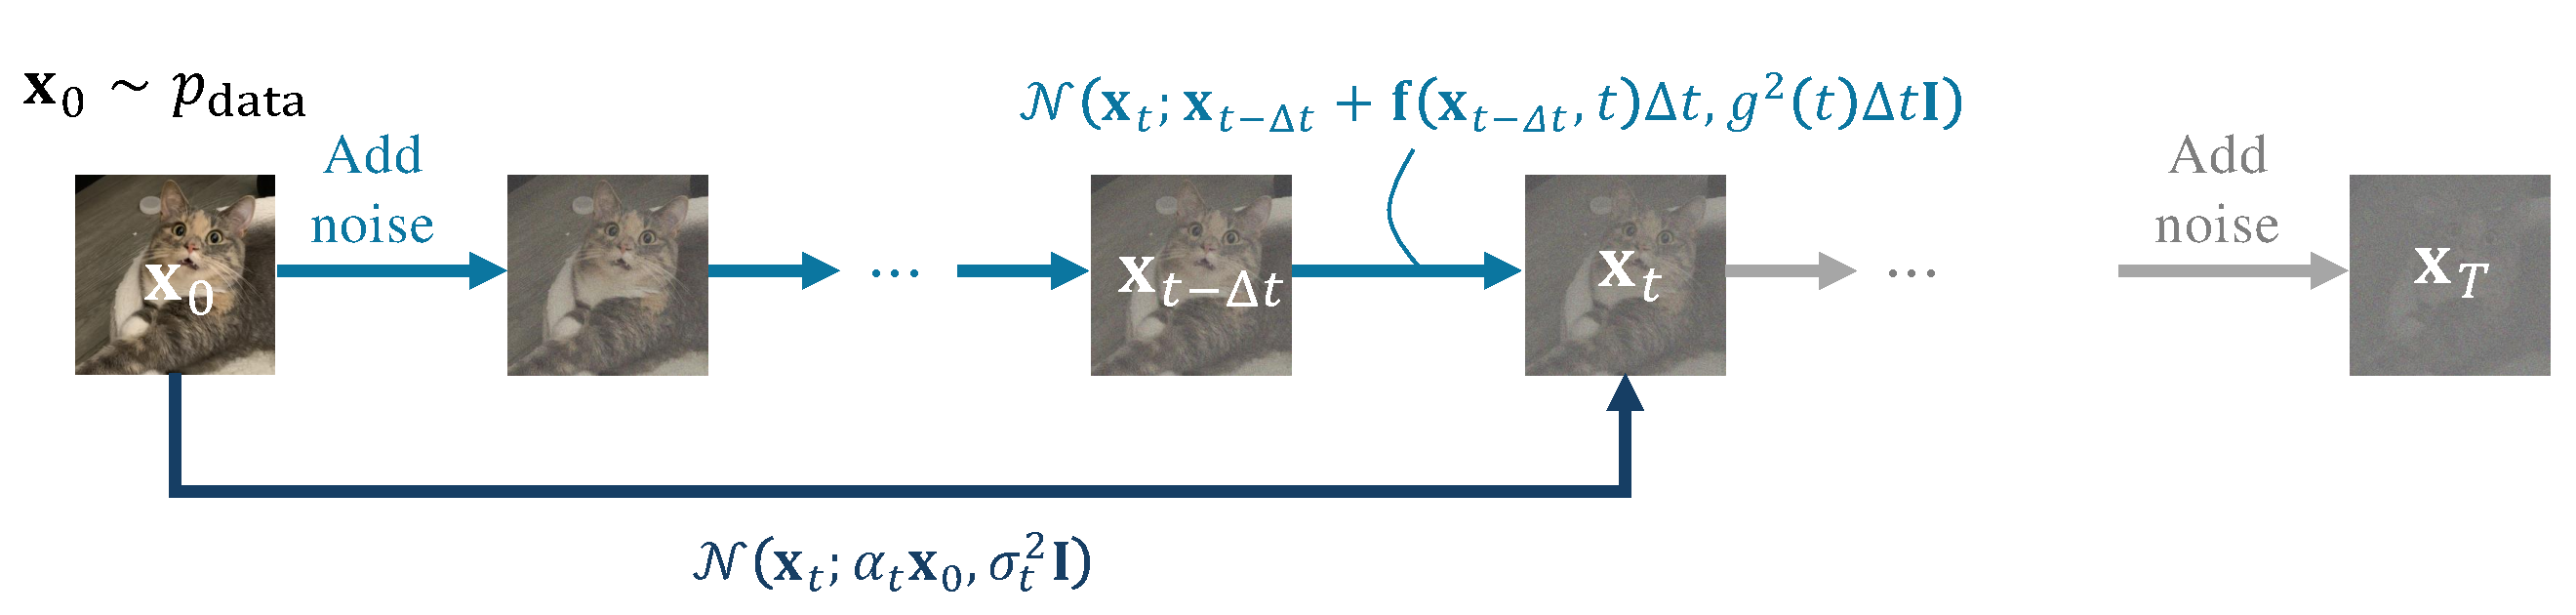
\includegraphics[width=\linewidth]{Images/PartB/vdm-sde.pdf}
    \caption{\textbfs{Illustration of Lemma~\ref{forward-sde}.} Incremental noise injection via continuous-time SDE ($\Delta t\to 0$) and direct perturbation of \Cref{eq:forward_kernel} are mathematically equivalent. \figcredit{Created by the authors.}}
    \label{fig:vdm-sde}
\end{figure}
\subsection{A General Affine Forward Process $p_t(\rvx_t |\rvx_0)$}
We begin with defining a general forward perturbation kernel:
\begin{equation}\label{eq:forward_kernel}
p_t(\rvx_t| \rvx_0) := \mathcal{N}\big(\rvx_t; \alpha_t \rvx_0, \sigma_t^2 \mathbf{I}\big),
\end{equation}
where $\rvx_0 \sim p_{\mathrm{data}}$, and $\alpha_t$, $\sigma_t$ are nonnegative scalar functions of $t \in [0,T]$ satisfying:
\begin{enumerate}
    \item[(i)] $\alpha_t > 0$ and $\sigma_t > 0$ for all $t \in (0,1]$ (allowing $\sigma_0 = 0$), and
    \item[(ii)] Typically, $\alpha_0 = 1$ and $\sigma_0 = 0$.
\end{enumerate}
That is, $\rvx_t \sim p_t(\rvx_t | \rvx_0)$ can be sampled as
\begin{equation*}
\rvx_t = \alpha_t \rvx_0 + \sigma_t \bm{\epsilon}, 
\qquad \bm{\epsilon} \sim \mathcal{N}(\mathbf{0}, \mathbf{I}).
\end{equation*}

This framework subsumes several well-known instances, including the VE (e.g., NCSN), the VP (e.g., DDPM), and the Flow Matching (FM) forward kernel~\citep{lipman2022flow, liu2022rectified}, which linearly interpolates between $\rvx_0$ and $\bm{\epsilon}$ (see later in \Cref{sec:flow-matching-framework}).
\begin{itemize}
\item \textbfs{VE (NCSN) Kernel:} $\alpha_t \equiv 1$, $\sigma_T \gg 1$;
\item \textbfs{VP (DDPM) Kernel:} $\alpha_t := \sqrt{1 - \sigma_t^2}$, so that $\alpha_t^2 + \sigma_t^2 = 1$;
\item \textbfs{FM Kernel:} $\alpha_t = 1 - t$, $\sigma_t = t$.
\end{itemize}

\subsection{Connection to Score SDE}
For Score SDE, specifying $ p_t(\rvx_t|\rvx_0) $ in a linear form naturally induces an SDE with affine coefficients, providing a more intuitive alternative to starting from drift and diffusion terms and solving ODEs for the moments (see \Cref{subsec:scoresde-perturbation-kernel}).

Given the forward perturbation kernel in \Cref{eq:forward_kernel}, the corresponding forward SDE takes the linear-in-$\rvx$ form as in \Cref{eq:forward-linear-sde}:
\begin{align*}
    \diff \rvx(t) = \underbrace{f(t)\rvx(t)}_{\rvf(\rvx(t), t)} \diff t + g(t) \diff\rvw(t),
\end{align*}
where $ f, g\colon [0,T] \rightarrow \mathbb{R} $ are real-valued functions of time. 
The coefficients $ f(t) $ and $ g(t) $ can be expressed analytically in terms of $ \alpha_t $ and $ \sigma_t $, as summarized in the following lemma.

\lemp{Forward Perturbation Kernel $\Leftrightarrow$ Linear SDE}{forward-sde}{ Define $\lambda_t:=\log\tfrac{\alpha_t}{\sigma_t}$ for $t\in(0,T]$.
Given the forward perturbation kernel
\[
\rvx_t=\alpha_t \rvx_0+\sigma_t \beps,\qquad \beps\sim\mathcal N(\mathbf 0,\rmI),
\]
the linear SDE
\[
\diff \rvx(t)=f(t) \rvx(t) \diff t+g(t) \diff\rvw(t),
\]
with coefficients 
\begin{align}\label{eq:kernel-sde-equiv}
\begin{aligned}
f(t)&=\frac{\diff}{\diff t}\log \alpha_t,\\
g^2(t)&=\frac{\diff \sigma_t^2}{\diff t}-2\frac{\diff}{\diff t}\log\alpha_t \sigma_t^2
       = -2\sigma_t^2 \frac{\diff}{\diff t}\lambda_t,
\end{aligned}
\end{align}
has the conditional transition $p_t(\rvx_t|\rvx_0)=\mathcal N \big(\rvx_t;\alpha_t\rvx_0,\sigma_t^2\rmI\big)$ for all $t\in(0,T]$.
Conversely, if a linear SDE has conditional transitions $\mathcal N(\rvx_t;\alpha_t\rvx_0,\sigma_t^2\rmI)$ so that $\alpha_t>0$ and $\sigma_t>0$ for all $t\in(0,T]$, then its coefficients satisfy \Cref{eq:kernel-sde-equiv} for $t\in(0,T]$.
}{From \Cref{subsec:scoresde-perturbation-kernel}, the proof matches the mean and covariance ODEs $\rvm'(t) = f(t)\rvm(t)$, $\rmP'(t) = 2f(t) \rmP(t) + g^2(t) \rmI$ with
$\rvm(t)=\alpha_t\rvx_0$ and $\rmP(t)=\sigma_t^2\rmI$ on $(0,T]$.}


\rmkb{To exactly match a Gaussian prior at the terminal time, the process must completely forget $\rvx_0$ and attain the target variance; this requires $\alpha_T=0$ and $\sigma_T^2$ equal to the prior variance.  

In the SDE formulation, one has
\[
\alpha_t=\exp \Big(\int_0^t f(u)\diff  u\Big).
\]
Thus, enforcing $\alpha_T=0$ at a finite $T$ forces
\[
\int_0^T f(u)\diff u=-\infty,
\]
meaning the drift must contract infinitely fast as $t\rightarrow T$.  
At the same time, the diffusion must diverge in order to maintain the prescribed variance, which is reflected by
\[
g^2(t)=\sigma_t^{2 \prime}-2\frac{\alpha_t'}{\alpha_t} \sigma_t^2  \rightarrow  \infty
\quad\text{as } t\rightarrow T.
\]

If $f$ and $g$ remain bounded on $[0,T]$, then necessarily $\alpha_T>0$ and a residual dependence on $\rvx_0$ remains. In that case, the Gaussian prior is attained only asymptotically: either in the limit $t\to T$ (without exact attainment) or exactly on an infinite horizon after an appropriate time reparameterization as $T\to\infty$.
}


From the above lemma, specifying the incremental noise injection via a linear SDE with coefficients $f(t)$ and $g(t)$ is mathematically equivalent to defining the perturbation kernel with parameters $\alpha_t$ and $\sigma_t$. In the diffusion model literature, these two viewpoints are used interchangeably. Therefore, we conclude:
\msg{Observation}{}{
Defining $p_t(\rvx_t | \rvx_0)$ is equivalent to specifying the linear SDE coefficients $f(t)$ and $g(t)$.
}


\subsection{Connection to Variational-Based Diffusion Model}\label{subsec:connection-vdm}
We revisit a core identity from DDPM, derived via Bayes’ rule:
\begin{align}\label{eq:ddpm-reverse-condition-kernel}
    p(\rvx_{t-\Delta t}|\rvx_t, \rvx) = p(\rvx_t|\rvx_{t-\Delta t}) \cdot \frac{p_{t-\Delta t}(\rvx_{t-\Delta t}|\rvx)}{p_t(\rvx_t|\rvx)},
\end{align}
for any $\rvx$ (usually $\rvx\sim p_{\mathrm{data}}$). This reverse conditional $ p(\rvx_{t-\Delta t} | \rvx_t, \rvx) $ is central to modeling, enabling both tractable training targets and efficient sampling.

Although DDPM typically defines the incremental kernel $p(\rvx_t|\rvx_{t-\Delta t})$ first, the accumulated transition $p_t(\rvx_t|\rvx_0)$ often provides a more interpretable and practical formulation, especially for the prior and loss design.

\paragraph{Deriving Transition Kernels.}
We now extend this to the continuous-time setting. Let $0 \leq t < s \leq T$ be two (continuous) time points. Given the perturbation kernel $p_t(\rvx_t|\rvx_0)$, we can compute the reverse conditional $p(\rvx_t|\rvx_s, \rvx)$ for any $\rvx$ by applying \Cref{eq:ddpm-reverse-condition-kernel}\footnote{This identity extends naturally to continuous time by treating $s$ as a general earlier time.}, using the forward kernel $p(\rvx_s|\rvx_t)$ as an intermediate. The following lemma summarizes this derivation, extending Lemma~\ref{ddpm-reverse-kernel} without assuming $\alpha_t^2 + \sigma_t^2 = 1$.

\lemp{Reverse Conditional Transition Kernels}{reverse-kernel}{
Let $0 \leq t < s \leq T$. The reverse \emph{conditional} transition kernel is:
\begin{equation*}
    p(\rvx_t|\rvx_s, \rvx) = \mathcal{N}\left(\rvx_t; \bm{\mu}(\rvx_s, \rvx; s, t), \sigma^2(s, t) \bfI\right),
\end{equation*}
where
\begin{align}\label{eq:p_backward_mean_var}
\begin{aligned}
    \bm{\mu}(\rvx_s, \rvx; s, t) := \frac{\alpha_{s|t} \sigma_t^2}{\sigma_s^2} \rvx_s + \frac{\alpha_t \sigma^2_{s|t}}{\sigma_s^2} \rvx, \quad
    \sigma^2(s, t) := \sigma^2_{s|t} \frac{\sigma_t^2}{\sigma_s^2}.
\end{aligned}
\end{align}
Here, $\alpha_{s|t}$ and $\sigma_{s|t}$ are defined as:
\begin{equation*}
    \alpha_{s|t} := \frac{\alpha_s}{\alpha_t}, \qquad \sigma^2_{s|t} := \sigma_s^2 - \alpha_{s|t}^2 \sigma_t^2.
\end{equation*}
}{
We first compute the forward transition kernel:
\begin{equation}\label{eq:zt_given_zs}
    p(\rvx_s|\rvx_t) = \mathcal{N}\left(\rvx_s; \alpha_{s|t} \rvx_t, \sigma^2_{s|t} \bfI\right).
\end{equation}
The reverse kernel then follows from Bayes’ rule, and since all involved distributions are Gaussian, the result can be derived by direct computation. For further details, see Appendix A of \citep{kingma2021variational}.
}


Although $p(\rvx_{t + \Delta t}|\rvx_t)$ and $p_t(\rvx_t|\rvx_0)$ are theoretically equivalent, $p_t(\rvx_t|\rvx_0)$ often takes a more central role. The step-wise transition in \Cref{eq:zt_given_zs} mainly serves to obtain a closed-form reverse kernel. Recent works~\citep{kingma2021variational} thus favor directly specifying $p_t(\rvx_t|\rvx_0)$ for its clarity and interpretability.



\paragraph{Reverse Process Modeling, Training, and Sampling.}  
The training objective (ELBO in \Cref{eq:ddpm-elbo}) and the modeling framework introduced in \Cref{sec:ddpm} remain applicable under our generalized setting. For clarity, we adopt the $\rvx$-prediction formulation, denoted by $\rvx_{\bm{\phi}}(\rvx_s, s)$, following~\citet{kingma2021variational}. However, the equivalent $\beps$-prediction perspective, represented by $\bm{\epsilon}_{\bm{\phi}}(\rvx_s, s)$, is also valid due to the relationship (as in \Cref{eq:ddpm-clean-noise})
\[
\rvx_s = \alpha_s \rvx_{\bm{\phi}}(\rvx_s, s) + \sigma_s \bm{\epsilon}_{\bm{\phi}}(\rvx_s, s),\quad \text{for any given } \rvx_s \sim q_s.
\]

\subparagraph{Modeling and Diffusion Loss $\mathcal{L}_{\text{diffusion}}$.}  
Similar to DDPM, the conditional distribution $p(\rvx_t|\rvx_s, \rvx)$ in \Cref{eq:p_backward_mean_var} motivates replacing the clean signal $\rvx$ with a learnable predictor $\rvx_{\bm{\phi}}(\rvx_s, s)$, yielding a parameterized reverse model of the form:
\begin{align}\label{eq:general-ddpm-sampling}
    p_{\bm{\phi}}(\rvx_t | \rvx_s) := \mathcal{N}\left(\rvx_t; \bm{\mu}_{\bm{\phi}}(\rvx_s, s, t), \sigma^2(s,t) \mathbf{I}\right),
\end{align}
with the mean parametrized as:
\[
    \bm{\mu}_{\bm{\phi}}(\rvx_s, s, t) = \frac{\alpha_{s|t} \sigma_t^2}{\sigma_s^2} \rvx_s + \frac{\alpha_t \sigma_{s|t}^2}{\sigma_s^2} \rvx_{\bm{\phi}}(\rvx_s, s).
\]
Given the forward kernel in \Cref{eq:forward_kernel}, the KL divergence in $\mathcal{L}_{\text{diffusion}}(\rvx; \bm{\phi})$ reduces to a weighted regression loss:
\begin{align}
\begin{aligned}
    \label{eq:snr-kl}
    \mathcal{D}_{\text{KL}}\big(p(\rvx_t|\rvx_s, \rvx_0)  \| p_{\bm{\phi}}(\rvx_t|\rvx_s)\big)  
    &= \frac{1}{2\sigma^2(s,t)} \left\| \bm{\mu}(\rvx_s, \rvx_0; s,t) - \bm{\mu}_{\bm{\phi}}(\rvx_s, s, t) \right\|_2^2 \\
    &= \frac{1}{2} \big(\text{SNR}(t) - \text{SNR}(s)\big) \left\| \rvx_0 - \rvx_{\bm{\phi}}(\rvx_s, s) \right\|_2^2,
\end{aligned}
\end{align}
where $\rvx_s = \alpha_s\rvx_0 + \sigma_s\bm{\epsilon}$, with $\rvx_0 \sim p_{\mathrm{data}}$, $\bm{\epsilon} \sim \mathcal{N}(\bm{0}, \rmI)$, and $\text{SNR}(s) := \alpha_s^2 / \sigma_s^2$ denotes the signal-to-noise ratio at time $s$.


\rmkb{
In \citep{kingma2021variational}, the authors study the continuous-time limit of \Cref{eq:snr-kl} as $t \to s$, yielding:
\begin{align*}
\mathcal{L}_{\text{VDM}}^\infty(\rvx_0) 
= -\frac{1}{2}  \mathbb{E}_{s, \bm{\epsilon} \sim \mathcal{N}(\bm{0}, \bfI)}  \text{SNR}'(s)  \big\| \rvx_0 - \rvx_{\bm{\phi}}(\rvx_s, s) \big\|_2^2.
\end{align*}
This setup also introduces a learnable noise schedule, and while it generalizes beyond continuous data, such extensions fall outside the scope of our current discussion.
}

\subparagraph{Sampling.}  
Sampling proceeds similarly to DDPM using the parameterized kernel from \Cref{eq:general-ddpm-sampling}:
\begin{align}\label{eq:general-ddpm-sampling-discrete}
    \rvx_t = \underbrace{\frac{\alpha_{s|t} \sigma_t^2}{\sigma_s^2} \rvx_s + \frac{\alpha_t \sigma_{s|t}^2}{\sigma_s^2} \rvx_{\bm{\phi}^\times}(\rvx_s, s)}_{\bm{\mu}_{\bm{\phi}^\times}(\rvx_s, t, s)} + \sigma_{s|t} \frac{\sigma_t}{\sigma_s} \bm{\epsilon}_s,\quad  \bm{\epsilon}_s \sim \mathcal{N}(\bm{0}, \rmI).
\end{align}



\clearpage
\newpage

\section{(Optional) Fokker–Planck Equation and Reverse-Time SDEs \\via Marginalization and Bayes’ Rule}\label{eq:heuristic-fpe-sde}
In this section, we offer a probabilistic perspective on the structure of the Fokker–Planck equation and the reverse-time SDE. By leveraging fundamental tools such as the marginalization trick and Bayes' rule, we illuminate the connection between the statistical formulation of stochastic processes and their corresponding differential equations.

We emphasize that the ``derivation'' presented here is not  mathematically rigorous proofs, but rather heuristic arguments intended to convey the underlying connections.


\subsection{Fokker-Planck Equation from the Marginalization of Transition Kernels}\label{subsec:fpe-reason}
Given the forward transition probability as in \Cref{eq:transition-forward-f-g}
\begin{align*}
    p(\mathbf{x}_{t+\Delta t} | \mathbf{x}_t) = \mathcal{N}\left(\mathbf{x}_{t+\Delta t}; \mathbf{x}_t + \mathbf{f}(\mathbf{x}_t, t)\Delta t, g^2(t)\Delta t \mathbf{I}\right),
\end{align*}
and the marginal distributions
\begin{align*}
    p_t(\mathbf{x}_t), \quad p_{t+\Delta t}(\mathbf{x}_{t+\Delta t}),
\end{align*}
we aim to derive the Fokker-Planck equation that governs the time evolution of the marginal distribution $p_t$.


\paragraph{Change of Variables.}
By the Markov property, the marginal distribution at time $t + \Delta t$ can be expressed as an integral over the previous state $\mathbf{x}_t$ (i.e., Chapman-Kolmogorov equation):
\begin{align*}
p_{t+\Delta t}(\rvx)
= \int \mathcal N \big(\rvx; \rvy+\rvf(\rvy,t)\Delta t, g^2(t)\Delta t \rmI\big) p_t(\rvy) \diff\rvy.
\end{align*}
 We introduce a new variable
\[
\rvu  :=  \rvy+\rvf(\rvy,t)\Delta t,
\]
so the Gaussian is centered at $\rvu$. For small $\Delta t$, this map is invertible with
\[
\rvy  =  \rvu-\rvf(\rvu,t)\Delta t+\mathcal O(\Delta t^2),
\quad
\Bigg|\det\frac{\partial \rvy}{\partial \rvu}\Bigg|
 = 1-(\nabla_\rvu \cdot\rvf)(\rvu,t) \Delta t+\mathcal O(\Delta t^2).
\]
Hence, change-of-variable formula leads us to:
\begin{align*}
    p_{t+\Delta t}(\rvx)
&= \int \mathcal N\left(\rvx;\rvu,g^2(t)\Delta t\rmI\right) \cdot
\\\quad\Big[p_t(\rvu)&-\Delta t \rvf(\rvu,t) \cdot \nabla_\rvu p_t(\rvu)
-\Delta t (\nabla_\rvu \cdot\rvf)(\rvu,t) p_t(\rvu)\Big] \diff\rvu
+\mathcal O(\Delta t^2),
\end{align*}

\paragraph{Taylor Expansion.}
For any smooth function $\phi:\R^D\to\R$ and scale $\sigma>0$,  
if $\rvz\sim\mathcal N(\bm{0},\rmI)$, the following approximation holds  
(known as the \emph{Taylor–Gaussian smoothing formula}):

\[
\int \mathcal N(\rvx;\rvu,\sigma^2\rmI) \phi(\rvu) \diff\rvu
=\E \left[\phi(\rvx+\sigma\rvz)\right]
=\phi(\rvx)+\frac{\sigma^2}{2} \Delta_\rvx\phi(\rvx)+\mathcal O(\sigma^4).
\]
This is because Taylor expansion for: 
\[
\phi(\rvx+\sigma\rvz)=\phi(\rvx)+\sigma\nabla_\rvx\phi(\rvx) \cdot \rvz+\frac{\sigma^2}{2}\rvz^\top\nabla_\rvx^2\phi(\rvx)\rvz+\mathcal O(\sigma^3)
\]
and $\E[\rvz]=\bm{0}$, $\E[\rvz\rvz^\top]=\rmI$.

Apply this with $\phi=p_t$, $\phi=\rvf \cdot \nabla_\rvu p_t$, and $\phi=(\nabla_\rvu \cdot\rvf) p_t$, and use $\sigma^2=g^2(t)\Delta t$, we can obtain
\[
\begin{aligned}
&p_{t+\Delta t}(\rvx) - p_t(\rvx)
\\=& -\Delta t \rvf(\rvx,t) \cdot \nabla_\rvx p_t(\rvx)
-\Delta t (\nabla_\rvx \cdot\rvf)(\rvx,t) p_t(\rvx)
+\frac{g^2(t)}{2}\Delta t \Delta_\rvx p_t(\rvx)
+\mathcal O(\Delta t^2) 
\\=&  - \Delta t \nabla_\rvx \cdot \big(\rvf(\rvx,t) p_t(\rvx)\big)
 + \frac{g^2(t)}{2} \Delta t \Delta_\rvx p_t(\rvx)
 + \mathcal O(\Delta t^2).
\end{aligned}
\]
Divide by $\Delta t$ and let $\Delta t\to0$ to obtain the Fokker–Planck equation.

In \Cref{subsec:rigorous-proof-fpe}, we present the It\^o--based derivation to complement the discrete--time view above.




\subsection{Why Does Reverse-Time SDE Take The Form?}\label{subsec:reverse-sde-reason}

The rigorous derivation of the reverse-time SDE is technical and requires delving into the properties of the Fokker-Planck equation. However, the form of the reverse-time SDE can be understood intuitively through Bayes' theorem. Here, we present a heuristic derivation to provide insight into why \Cref{eq:sde_backward} takes its form, with the appearance of score functions\footnote{This derivation is inspired by the approach in \href{https://alexxthiery.github.io/notes/reverse_and_tweedie/reverse_and_tweedie.html}{this post}.}. 


\paragraph{Using Bayes' Rule for Inversion.} 
Our goal is to determine the reverse-time transition kernel by first considering the discrete-time case:
\[
p(\rvx_t | \rvx_{t+\Delta t}),
\]
and then taking $\Delta t \rightarrow 0$ to obtain the continuous-time formulation.
Using Bayes' theorem, we express:
\begin{align}\label{eq:reverse-sde-bayes-discrete}
    p(\rvx_t | \rvx_{t+\Delta t}) 
    &= p(\rvx_{t+\Delta t} | \rvx_t) \frac{p_t(\rvx_t)}{p_{t+\Delta t}(\rvx_{t+\Delta t})} \nonumber \\
    &= p(\rvx_{t+\Delta t} | \rvx_t) \exp\left(\log p_t(\rvx_t) - \log p_{t+\Delta t}(\rvx_{t+\Delta t})\right).
\end{align}

The forward transition kernel is assumed to be as in \Cref{eq:transition-forward-f-g}:
\begin{equation*}
p(\rvx_{t+\Delta t} | \rvx_t) = \mathcal{N}\left(\rvx_{t+\Delta t}; \rvx_t + \rvf(\rvx_t, t)\Delta t, g^2(t)\Delta t \mathbf{I}\right)
\end{equation*}

\paragraph{Taylor Expansion.} 
To handle the exponential term, we apply a first-order Taylor expansion. The key insight is to expand around the point $(\rvx_t, t)$ in both space and time:
\begin{align*}
    \log p_{t+\Delta t}(\rvx_{t+\Delta t}) &= \log p_t(\rvx_t) + \nabla_{\rvx} \log p_t(\rvx_t) \cdot (\rvx_{t+\Delta t} - \rvx_t) \nonumber \\
    &\quad + \frac{\partial \log p_t(\rvx_t)}{\partial t} \Delta t + \mathcal{O}(\|\rvh\|_2^2) 
\end{align*}
where $\rvh := (\rvx_{t+\Delta t} - \rvx_t, \Delta t)$. Therefore:
\begin{align}
    \log p_t(\rvx_t) - \log p_{t+\Delta t}(\rvx_{t+\Delta t}) &= -\nabla_{\rvx} \log p_t(\rvx_t) \cdot (\rvx_{t+\Delta t} - \rvx_t) \nonumber \\
    &\quad - \frac{\partial \log p_t(\rvx_t)}{\partial t} \Delta t + \mathcal{O}(\|\rvh\|_2^2) \label{eq:log-difference}
\end{align}

For the forward process with finite drift and diffusion, we have $\mathbb{E}[\|\rvx_{t+\Delta t} - \rvx_t\|_2^2] = \mathcal{O}(\Delta t)$, which ensures that the remainder term is $\mathcal{O}((\Delta t)^2)$ in expectation.

\paragraph{Substituting into the Reverse Transition.}
Substituting equations \Cref{eq:transition-forward-f-g} and \Cref{eq:log-difference} into \Cref{eq:reverse-sde-bayes-discrete}:
\begin{align*}
    &p(\rvx_t | \rvx_{t+\Delta t}) \nonumber \\
    = &\frac{1}{(2\pi g^2(t) \Delta t)^{D/2}} \exp\left(-\frac{\|\rvx_{t+\Delta t} - \rvx_t - \rvf(\rvx_t, t) \Delta t\|_2^2}{2 g^2(t) \Delta t}\right) \nonumber \\
    &\qquad \cdot \exp\left(-\nabla_{\rvx} \log p_t(\rvx_t) \cdot (\rvx_{t+\Delta t} - \rvx_t) - \frac{\partial \log p_t(\rvx_t)}{\partial t} \Delta t + \mathcal{O}((\Delta t)^2)\right). 
\end{align*}
\paragraph{Algebraic Manipulation.}
The key step is to complete the square in the exponent. We have:
\begin{align*}
    &-\frac{\|\rvx_{t+\Delta t} - \rvx_t - \rvf(\rvx_t, t) \Delta t\|_2^2}{2 g^2(t) \Delta t} - \nabla_{\rvx} \log p_t(\rvx_t) \cdot (\rvx_{t+\Delta t} - \rvx_t) \nonumber \\
    = &-\frac{\left[\|\rvx_{t+\Delta t} - \rvx_t - \rvf(\rvx_t, t) \Delta t\|_2^2 + 2 g^2(t) \Delta t \nabla_{\rvx} \log p_t(\rvx_t) \cdot (\rvx_{t+\Delta t} - \rvx_t)\right]}{2 g^2(t) \Delta t} 
\end{align*}
Let $\boldsymbol{\delta} := \rvx_{t+\Delta t} - \rvx_t$ and $\boldsymbol{\mu} := \rvf(\rvx_t, t) \Delta t$. Then:
\begin{align*}
    &\|\boldsymbol{\delta} - \boldsymbol{\mu}\|_2^2 + 2 g^2(t) \Delta t \nabla_{\rvx} \log p_t(\rvx_t) \cdot \boldsymbol{\delta} \nonumber \\
    = &\|\boldsymbol{\delta}\|_2^2 - 2\boldsymbol{\delta} \cdot \boldsymbol{\mu} + \|\boldsymbol{\mu}\|_2^2 + 2 g^2(t) \Delta t \nabla_{\rvx} \log p_t(\rvx_t) \cdot \boldsymbol{\delta} \nonumber \\
    = &\|\boldsymbol{\delta}\|_2^2 - 2\boldsymbol{\delta} \cdot [\boldsymbol{\mu} - g^2(t) \Delta t \nabla_{\rvx} \log p_t(\rvx_t)] + \|\boldsymbol{\mu}\|_2^2 \nonumber \\
    = &\|\boldsymbol{\delta} - [\boldsymbol{\mu} - g^2(t) \Delta t \nabla_{\rvx} \log p_t(\rvx_t)]\|_2^2 - \|g^2(t) \Delta t \nabla_{\rvx} \log p_t(\rvx_t)\|_2^2 
\end{align*}
Substituting back:
\begin{align*}
    &\|\boldsymbol{\delta} - [\rvf(\rvx_t, t) \Delta t - g^2(t) \Delta t \nabla_{\rvx} \log p_t(\rvx_t)]\|_2^2 \nonumber \\
    = &\|\rvx_{t+\Delta t} - \rvx_t - [\rvf(\rvx_t, t) - g^2(t) \nabla_{\rvx} \log p_t(\rvx_t)] \Delta t\|_2^2. 
\end{align*}
Therefore,
\begin{align*}
    p(\rvx_t | \rvx_{t+\Delta t}) 
    =~&\frac{1}{(2\pi g^2(t) \Delta t)^{D/2}} \nonumber \\
    \quad &\cdot \exp\left(-\frac{\|\rvx_{t+\Delta t} - \rvx_t - [\rvf(\rvx_t, t) - g^2(t) \nabla_{\rvx} \log p_t(\rvx_t)] \Delta t\|_2^2}{2 g^2(t) \Delta t}\right) \nonumber \\
    \quad &\cdot \exp(\mathcal{O}(\Delta t)) \nonumber \\
    =~&\mathcal{N}\left(\rvx_t; \rvx_{t+\Delta t} - [\rvf(\rvx_t, t) - g^2(t) \nabla_{\rvx} \log p_t(\rvx_t)] \Delta t, g^2(t) \Delta t \mathbf{I}\right) \nonumber \\
    \quad &\cdot (1 + \mathcal{O}(\Delta t)).
\end{align*}
The additional term $\|g^2(t) \Delta t \nabla_{\rvx} \log p_t(\rvx_t)\|_2^2$ from completing the square is $\mathcal{O}((\Delta t)^2)$ and can be absorbed into the error term. Similarly, the time derivative term $\frac{\partial \log p_t(\rvx_t)}{\partial t} \Delta t$ is $\mathcal{O}(\Delta t)$ and will vanish in the continuous limit.

\paragraph{Taking $\Delta t \rightarrow 0$ Limit.}
As $\Delta t \approx 0$, under smoothness assumptions, the following approximations hold:
\begin{align*}
    \rvf(\rvx_t, t) &\approx \rvf(\rvx_{t+\Delta t}, t+\Delta t), \\
    g(t) &\approx g(t+\Delta t), \\
    \nabla_{\rvx} \log p_t(\rvx_t) &\approx \nabla_{\rvx} \log p_{t+\Delta t}(\rvx_{t+\Delta t})  = \rvs(\rvx_{t+\Delta t}, t+\Delta t).
\end{align*}
Using these approximations and some rearrangements, we obtain:
\begin{align*}
    &p(\rvx_t | \rvx_{t+\Delta t}) \\ \approx &\frac{1}{(2\pi g^2(t) \Delta t)^{D/2}}  \exp \Bigg(
            \\ &-\frac{\Big\|\rvx_{t} - \Big(\rvx_{t+\Delta t} - \big[\rvf(\rvx_{t+\Delta t}, t+\Delta t) - g^2({t+\Delta t}) \rvs(\rvx_{t+\Delta t}, t+\Delta t)\big] \Delta t\Big) \Big\|_2^2 }{2 g^2(t+\Delta t) \Delta t} \\
            &\Bigg).
\end{align*}
This implies that $p(\rvx_t | \rvx_{t+\Delta t})$ is roughly a normal distribution with:
\begin{align*}
    \text{\textbfs{Mean:}} &  \quad\rvx_{t+\Delta t} - \big[\rvf(\rvx_{t+\Delta t}, t+\Delta t) - g^2(t+\Delta t) \rvs (\rvx_{t+\Delta t}, t+\Delta t)\big] \Delta t, \\
    \text{\textbfs{Covariance:}} & \quad g^2(t+\Delta t) \Delta t \mathbf{I}.
\end{align*}
Taking the limit as $\Delta t \rightarrow 0$, we ``derive'' the reverse-time continuous SDE given in \Cref{eq:sde_backward}.






\clearpage
\newpage

\section{Closing Remarks}


This chapter marked a pivotal moment in our journey, unifying the discrete-time diffusion processes from the variational and score-based perspectives into a single, elegant continuous-time framework. We demonstrated that both DDPM and NCSN can be understood as discretizations of Stochastic Differential Equations (SDEs) with different drift/volatility coefficients.

The cornerstone of this framework is the existence of a corresponding reverse-time SDE, which formally defines a generative process that reverses the noise corruption. Crucially, the drift of this reverse process depends on a single unknown quantity: the score function, $\nabla_{\mathbf{x}}\log{p_{t}(\mathbf{x})}$, of the marginal data distributions at every point in time. This insight solidifies the score function's central role in generative modeling.

Furthermore, we introduced a purely deterministic counterpart, the Probability Flow Ordinary Differential Equation (PF-ODE), whose solution trajectories evolve along the same marginal densities $\{p_{t}\}$ as the SDEs. This remarkable consistency is guaranteed by the underlying Fokker-Planck equation. The profound implication is that the complex task of generation is fundamentally equivalent to solving a differential equation. Training reduces to learning the score function that defines the equation's vector field, while sampling becomes a problem of numerical integration.

The introduction of the PF-ODE, a purely deterministic flow, provides a powerful bridge to the third and final perspective on diffusion models. This concept of learning a deterministic transformation governed by a velocity field is the central principle of recent major family of generative models. In the next chapter, we will:
\begin{enumerate}
    \item Explore this flow-based perspective, starting from its origins in Normalizing Flows and Neural ODEs.
    \item Show how this viewpoint leads to the modern framework of Flow Matching, which directly learns a velocity field to transport samples between distributions.
\end{enumerate}

Ultimately, we will see how the deterministic PF-ODE, which we derived from stochastic principles, can be constructed and generalized from this entirely different, flow-based origin, completing our unified picture of diffusion modeling.



% \msg{}{From the derivation, we can conceptually understand that Bayes' rule in \Cref{eq:reverse-sde-bayes-discrete},
% \begin{align*}
%     p(\rvx_t |\rvx_{t+\Delta t})  
%     = p(\rvx_{t+\Delta t} |\rvx_t) \cdot \frac{p_t(\rvx_t)}{p_{t+\Delta t}(\rvx_{t+\Delta t})},
% \end{align*}
% serves as a discrete-time approximation of the reverse-time SDE, with an approximation error of order $ \abs{\Delta t} $.
% }



% \newpage

% \subsection{A Conceptual Variational Derivation of the Shared Fokker–Planck Equation for Forward and Reverse Processes}\label{subsec:conceptual-same-fokker-planck}

% In \Cref{subsec:fpe-sde-ode}, we observed that the reverse-time SDE is constructed to match the marginal distributions of the forward SDE, thereby mapping the noise distribution back to the data distribution. In this section, we develop an intuitive understanding of why the reverse-time dynamics—at the level of transition probabilities—should mirror those of the forward process, viewed from a variational perspective in discrete time.



% We begin by defining the forward transition kernel as follows:
% \begin{align*}
%     p(\rvx_{t+\Delta t} | \rvx_t) = \mathcal{N}\left(\rvx_{t+\Delta t}; \rvx_t + \rvf(\rvx_t, t)\Delta t, g^2(t)\Delta t \mathbf{I}\right),
% \end{align*}
% where the initial distribution is given by $p_0 = p_{\mathrm{data}}$.

% \paragraph{Forward Process.}
% We revisit the formulation in \Cref{subsec:fpe-reason}, introducing slightly revised notations for consistency with the reverse process discussed later. Given the specified forward transition kernel, we can compute the conditional distribution $p_t(\rvx_t|\rvx_0)$, which in turn induces the marginal distribution at time $t$:
% \begin{align*}
% p_{t}^{\text{fwd}}(\rvx_t) := \int p_t(\rvx_t|\rvx_0)  p_{\mathrm{data}}(\rvx_0)  \diff\rvx_0.
% \end{align*}

% From the Chapman-Kolmogorov equation, the forward evolution satisfies
% \begin{align*}
% p_{t+\Delta t}^{\text{fwd}}(\rvx_{t+\Delta t}) = \int p(\rvx_{t+\Delta t}|\rvx_t) p_{t}^{\text{fwd}}(\rvx_t) \diff\rvx_t.
% \end{align*}
% Therefore, we can obtain the 
% \begin{align*}
% p_{t+\Delta t}^{\text{fwd}}(\rvx) - p_{t}^{\text{fwd}}(\rvx) = \left[-\nabla \cdot [\rvf(\rvx, t) p_t^{\text{fwd}}(\rvx)] + \frac{g^2(t)}{2} \nabla^2 p_t^{\text{fwd}}(\rvx)\right] \Delta t + \mathcal O(\Delta t^2).
% \end{align*}

% \paragraph{Reverse Process.}

% The reverse process evolves backward in time from the terminal distribution. Starting with $p_{0}^{\text{rev}} := p_{T}^{\text{fwd}}$, by Bayes' rule, we have when $\Delta t \approx 0$
% \begin{align*}
%     &p(\rvx_{t-\Delta t}|\rvx_t) \\
%     =~&p(\rvx_{t}|\rvx_{t-\Delta t}) \frac{p_{t-\Delta t}^{\text{fwd}}(\rvx_{t-\Delta t})}{p_t^{\text{fwd}}(\rvx_t)} \\
%     =~&p(\rvx_{t}|\rvx_{t-\Delta t}) \exp\left(\log p_{t-\Delta t}^{\text{fwd}}(\rvx_{t-\Delta t}) - \log p_{t}^{\text{fwd}}(\rvx_{t})\right) \\
%     =~&\mathcal{N}\left(\rvx_{t-\Delta t}; \rvx_{t} - \big[\rvf(\rvx_{t}, t) - g^2(t) \rvs (\rvx_{t}, t)\big] \Delta t, g^2(t) \Delta t \mathbf{I}\right) \nonumber   \cdot (1 + \mathcal{O}(\Delta t)),
% \end{align*}
% where $\rvs(\rvx_t, t) = \nabla \log p_t^{\text{fwd}}(\rvx_t)$ is the score function.
% With this, it induces the reverse perturbation kernel $p^{\text{rev}}(\rvx_t|\rvx_0)$ and the reverse marginal distribution: 
% \begin{align*}
% p_{t}^{\text{rev}}(\rvx_t) &:= \int p^{\text{rev}}(\rvx_t|\rvx_0) p_{0}^{\text{rev}}(\rvx_0)\diff\rvx_0.
% \end{align*}

% By the Markov property and the marginal consistency condition (as formalized by the Chapman–Kolmogorov equation), the reverse-time marginal satisfies
% \begin{align*}
% p_{t-\Delta t}^{\text{rev}}(\rvx_{t-\Delta t}) = \int p(\rvx_{t-\Delta t}|\rvx_t)  p_{t}^{\text{rev}}(\rvx_t)  \diff\rvx_t.
% \end{align*}
% Following analogous steps to the forward case, we substitute the reverse transition kernel and write $\rvx= \rvx_{t-\Delta t}$ and $\rvy = \rvx_t$:
% \begin{align*}
% p_{t-\Delta t}^{\text{rev}}(\rvx) \approx \int \mathcal{N}(\rvx; \mathbf{y} - [\rvf(\mathbf{y}, t) - g^2(t) \rvs(\mathbf{y}, t)] \Delta t, g^2(t)\Delta t \mathbf{I}) p_t^{\text{rev}}(\mathbf{y}) \diff\mathbf{y}
% \end{align*}
% Similar to the forward process computation, we can derive
% \begin{align*}
% &p_{t-\Delta t}^{\text{rev}}(\rvx) - p_{t}^{\text{rev}}(\rvx) \\\approx &\left[\nabla \cdot [(\rvf(\rvx, t) - g^2(t) \rvs(\rvx, t)) p_t^{\text{rev}}(\rvx)] + \frac{g^2(t)}{2} \nabla^2 p_t^{\text{rev}}(\rvx)\right] (-\Delta t) + \mathcal{O}(\Delta t^2),
% \end{align*}
% by applying the change of variables $\mathbf{z} = \mathbf{y} - [\rvf(\mathbf{y}, t) - g^2(t) \rvs(\mathbf{y}, t)] \Delta t$, Taylor expansion, and Gaussian convolution.


% \paragraph{Equivalence Under Time Reversal.}

% The forward and reverse discretizations are mathematically equivalent representations of the same stochastic process evolving in opposite time directions. Specifically, when we set:
% \begin{align*}
%     p_t^{\text{rev}}(\rvx) = p_{T-t}^{\text{fwd}}(\rvx).
% \end{align*}
% Then both discretizations describe the same underlying Fokker-Planck dynamics, with the reverse process providing a path from the terminal distribution back to the initial distribution.

% This equivalence is fundamental to diffusion models and score-based generative modeling, where the reverse process enables sampling from complex distributions by reversing a simple forward diffusion process.

